\pdfoptionpdfminorversion=7
\documentclass[
	10pt, % font size (default is 10pt)
	english, % language
	twoside % documents can be either one sided (eg articles) or two sided (eg books), affects margins and stuff
]{article}

\def \title {Controlling Behavior in Animals and Robots}
\def \subtitle {Mini-project}
\def \author {James Bardet -- Nicolas Furrer -- Claire Meyer}
\def \creator {Claire Meyer}
\def \institution {EPFL}
\def \professor {Pavan Ramdya}
\def \course {Controlling Behavior in Animals and Robots}
\def \place {Écublens}
\def \subject {bioscience}
\def \sciper {287045 -- 215236 -- 204326}
\def \tags {project}


%%%%%%%%%%%%%%%%%%%%%%%%%%%%%%%%
%% PLATFORM DEPENDANT CONDITIONS
%%%%%%%%%%%%%%%%%%%%%%%%%%%%%%%%

\usepackage{ifplatform}
% allows to detect which os is running the compilation

%%%%%%%%%%%%%%%%%%%%%%%
%% INTERNATIONALIZATION
%%%%%%%%%%%%%%%%%%%%%%%

\usepackage{babel}
% allows the internationalization of the document, language specified in the document class
% should be placed soon after the \documentclass command, so that all the other packages loaded afterwards know the used language

\usepackage[T1]{fontenc} 
% defines the font encoding
% is used when in need of non-english caracters 
% (if the document is only english, then no need for it, the default font encoding is good)
% allows for automatic hyphenation of accentuated words
% allows for successful search of accentuated words in pdf
% allows for successful copy pasting of accentuated words from pdf

\usepackage[utf8]{inputenc}
% defines the character encoding


%%%%%%%%%%%%%%
%% MATHEMATICS
%%%%%%%%%%%%%%

\usepackage{mathtools}
% simplifies the usage of complicated mathematical formulae
% loads the amsmath package, fixes some of its quirks and adds some useful settings, symbols, and environments to it

\setcounter{MaxMatrixCols}{20}

\usepackage{siunitx}

\usepackage{empheq}


%%%%%%%
%% TEXT
%%%%%%%

\usepackage{textcomp}
% provides extra symbols, e.g. arrows like \textrightarrow, various currencies (\texteuro,...), things like \textcelsius and many others

\usepackage{alltt}
% processes text as if by a typewriter (verbatim), BUT still recognizes commands

\usepackage{cprotect}


%%%%%%%%%%%%%
%% HYPERLINKS
%%%%%%%%%%%%%

\usepackage[
	bookmarks=true, % shows the bookmarks bar when displaying the document
	bookmarksnumbered=false, % put section numbers in bookmarks
	pdftoolbar= true, % shows or hide Acrobat?s toolbar
	pdfmenubar=true, % shows or hide Acrobat?s menu
	unicode=true, % allows to use characters of non-Latin based languages in Acrobat?s bookmarks
	%%%%%%%%%%%%%%%%%
	colorlinks=true, % surround the links by color frames (false) or colors the text of the links (true)
	linkcolor=blue, % color of internal links (sections, pages, etc.)
	citecolor=blue, % color of citation links (bibliography)
	filecolor=blue, % color of file links
	urlcolor=blue, % color of URL links (mail, web)
	anchorcolor=black, % color of anchor text
	menucolor=black, % color for menu links
	linktoc=section, % defines which part of an entry in the table of contents is made into a link (none, section, page, all)
	%%%%%%%%%%%%%%%%%
	pdffitwindow=false, % resizes document window to fit document size
	pdfnewwindow=true, % define if a new PDF window should get opened when a link leads out of the current document, the option is ignored if the link leads to an http/https address
	pdfstartpage={1}, % page at which PDF document opens
	pagebackref=false, % activate back references inside bibliography, must be specified as part of the \usepackage{} statement, must be set to false to work with biblatex
	%%%%%%%%%%%%%%%%%
	pdftitle={\subtitle}, %	defines the title that gets displayed in the "Document Info" window of Acrobat
	pdfauthor={\author}, % the name of the PDF?s author, works like the one above
	pdfsubject={\subject}, % subject of the document, it works like the one above
	pdfcreator={\creator}, % creator of the document, it works like the one above
	pdfproducer={TeXstudio}, % producer of the document, it works like the one above
	pdfkeywords={\tags}, % list of keywords, separated by commas, example below
]{hyperref}
% provides LaTeX the ability to create hyperlinks within the documen


%%%%%%%%%%%%%
%% APPEARANCE
%%%%%%%%%%%%%

\usepackage[
dvipsnames, % defines the use of the colors from the dvips / SVG set
table, % allows the use of colors in tables
]{xcolor}
% provides both foreground and background color management, has to be loaded before pdfpages to avoid option clash

\usepackage{pdfrender}



%%%%%%%%%%%%
%% PDF PAGES
%%%%%%%%%%%%

\usepackage{pdfpages}
% allows the insertion of pdf pages, has to be loaded after xcolor package to avoid option clash


%%%%%%%%%
%% FLOATS
%%%%%%%%%

\usepackage{floatrow}
% loads both rotfloat and float packages, rotfloat loads both rotating and float packages
% should not be loaded WITH any of the internally loaded packages
% provides commands to define new floats of various styles and new environments which are rotated by 90 or 270 degrees
% improves the interface for defining floating objects such as figures and tables
% pro­vides th H float mod­i­fier op­tion
% allows to change the font size inside tables


%%%%%%%%%
%% TABLES
%%%%%%%%%

\usepackage{multirow}
% provides the command needed for spanning rows

% defines column types for colored tables
\newcommand*{\arraycolor}[1]{\protect\leavevmode\color{#1}}
\newcolumntype{A}{>{\columncolor{LimeGreen!50!white}}m{4cm}}
\newcolumntype{B}{>{\columncolor{LimeGreen!50!white}}m{2cm}}
\newcolumntype{C}{>{\columncolor{LimeGreen!50!white}}m{0.7cm}}
\newcolumntype{D}{>{\columncolor{Yellow!50!white}}m{0.5cm}}
\newcolumntype{E}{>{\columncolor{LimeGreen!50!white}}m{6cm}}
\newcolumntype{F}{>{\columncolor{Red!50!white}}m{6cm}}
\newcolumntype{G}{>{\columncolor{LimeGreen!50!white}}m{7cm}}
\newcolumntype{H}{>{\columncolor{LimeGreen}}m{3cm}}

\floatsetup[table]{capposition=top}
% for table captions on top


%%%%%%%%%%
%% FIGURES
%%%%%%%%%%

\usepackage{graphicx}
% allows the importation of external graphics (pdf, png and jpg)

\graphicspath{{img/}}
% sets the path to external graphics

\usepackage{epstopdf}
% converts EPS to PDF

\usepackage{svg}
% allows the automated integration of SVG graphics into LATEX documents

\usepackage{caption}
% provides many ways to customise the captions in floating environments

\usepackage{subcaption}


%%%%%%%%%%%
%% LISTINGS
%%%%%%%%%%%

%\usepackage{minted}
%\usepackage{inconsolata}
%\usemintedstyle{monokai}
%\definecolor{bg}{HTML}{282828}
%\setminted{xleftmargin=10pt, linenos=true, fontsize=\footnotesize, tabsize=4, bgcolor=bg}
%\usepackage{tcolorbox}
%\BeforeBeginEnvironment{minted}{\begin{tcolorbox}[colback=bg, colframe=gray, boxsep=0mm]}%
%	\AfterEndEnvironment{minted}{\end{tcolorbox}}%
%
%% change the size and color of the line numbers
%\renewcommand\theFancyVerbLine{\color{gray}\arabic{FancyVerbLine}}


%%%%%%%%%%%%%%%%%%%%%%%%%%
%% BIBLIOGRAPHY MANAGEMENT
%%%%%%%%%%%%%%%%%%%%%%%%%%

\usepackage[
backend=biber,
defernumbers=true,
style=numeric,
backref=true
]{biblatex}
% processes bibliography information, provides an easy and flexible interface and a good language localization 
\addbibresource{bibliography.bib}
% specifies the bibtex data file

\usepackage{csquotes}
% provides advanced facilities for inline and display quotations
% ensures that quoted texts are typeset according to the rules of the main language when using babel or polyglossia with biblatex


%%%%%%%%%%%%%%
%% PAGE LAYOUT
%%%%%%%%%%%%%%

% \usepackage{showframe}
% renders a frame marking the margins of the document

\usepackage[
a4paper, % page size (default is letter, USA standard)
portrait, % page orientation (default is portrait)
top=2.5cm, 
bottom=2.5cm, 
inner=2.3cm, 
outer=2.3cm % specifies the margins
]{geometry}
% allows the customization of document layout

\usepackage{fancyhdr}
% allows fine customization of headers and footers (construction and usage)s
	\setlength{\headheight}{\baselineskip} % height of the header
	\pagestyle{fancy} % page style
	
	\lhead[\course]{\course}
	\chead[]{}
	\rhead[\rightmark]{\rightmark} % current section name printed like "1.6. THIS IS THE SECTION TITLE"
	% headers, [<even output>]{<odd output>}
	
	\lfoot[\thepage]{}
	\cfoot[]{}
	\rfoot[]{\thepage}
	% footers, [<even output>]{<odd output>}

\usepackage{lastpage}
% provides with internal link to last page (\pageref{LastPage})

\setcounter{secnumdepth}{5} % determines up to what level the sectioning titles are numbered
\setcounter{tocdepth}{4} % determines to which level the sectioning commands are printed in the ToC

\setlength{\parindent}{0 cm} % deletes indentation at each new paragraph
\numberwithin{equation}{section} % section numerotation of equation 
\numberwithin{figure}{section} 
\numberwithin{table}{section} 
%\numberwithin{listing}{section}

\begin{document}
	%%%%%%%%%%%%%%%
	%% RENEWCOMMAND
	%%%%%%%%%%%%%%%
	\renewcommand\labelitemi{\textbullet}
	\renewcommand\labelitemii{$\circ$}
	\renewcommand\labelitemiii{$\star$}
	% redefines the itemizing symbols for the itemize environment, 
	% cannot redefine the 4th lvl, 
	% cannot have more than 4 lvls,
	% in french, by default, it's all dashes...
	
	%%%%%%%%%%%%%
	%% TITLE PAGE
	%%%%%%%%%%%%%
	\hypersetup{pageanchor=false}
\begin{titlepage}
	
	\begin{center} 
		\includesvg[height=0.8cm]{epfl_logo} 
	\end{center}
	
	\vfill
	
	\begin{center}
		\rule{\linewidth}{1mm}
		\bigskip
		
		\Huge \title\\
		\bigskip
		
		\Large \subtitle\\
		\bigskip
		
		\rule{1cm}{0.3mm}\\
		\bigskip		
		
		\large \author\\
		\bigskip
		
		\rule{\linewidth}{1mm}
		\vfill
		
		\small \institution \\


		\vfill
		
		\small{
			\begin{tabular}{l@{: }l}
				Professor &\professor\\
				Course &\course\\
				Last update &\today\\
				Place &\place\\
				SCIPERs &\sciper\\
			\end{tabular} 
		}
	\end{center} 
\end{titlepage}
\hypersetup{pageanchor=true}
\newpage
	
	%%%%%%%%%%%%%%%%%%%
	%% TABLE OF CONTENT
	%%%%%%%%%%%%%%%%%%%
	\setcounter{page}{1} % beginning of page numeration here
	\tableofcontents
	\newpage
	
	%%%%%%%%
	%% INPUT
	%%%%%%%%
	\section{Introduction}

The ventral nerve cord (VNC) is a major structure of the invertebrate central nervous system, including that of \textit{Drosophila}.
It runs down the ventral plane of the organism, and is the insect motor control center.
It contains both descending neurons (DNs) and ascending neurons (ANs).
The former have their bodies and dendrites in the brain, and their axons projecting through the VNC, while it is the reverse for ANs.

\vspace{\baselineskip}

It has been theoretically hypothesized that artificially driving a small set of DNs could flexibly elicit multiple complex behaviors in individuals~\cite{ijspeert2007}, like swimming and walking.
In practice, the hypothesis has not been testable before transgenic strains of \textit{Drosophila} were made available in 2014~\cite{bidaye2014} and 2018~\cite{namiki2018}, allowing for DNs neuron targeting for studies of anatomy and function.
It has then been proven that individual DNs activation can trigger distinct behavior like backward walking, in experiments on single DN stimulation.

\vspace{\baselineskip}

More recently, technological advances such as two-photon imaging have allowed the simultaneous recording of multiple neurons at once~\cite{chen2018}.
Using this technique, an experiment consisting of the simultaneous recording of 123 DNs of \textit{Drosophila} was run, while the subject flies were freely moving on an air-suspended spherical treadmill.
The data gathered thus consist of spontaneous behavioral observations (video recordings), associated with the respective neural data (two-photon imaging of DNs) and kinematic data (relative joint positions and angles of leg segments).

\vspace{\baselineskip}

Because the data gathered is simultaneous, it allows to try to link specific behaviors with specific neural activity.
It is an observational study, though, so that causation cannot be inferred, only correlation (if present).
Thus, the goal of this project is to determine possible correlations between DNs of \textit{Drosophila} and some high level behaviors of the insect, and see if classification allows for behavioral prediction.

\newpage

	\section{Data preprocessing}

As previously stated, the data gathered is three-fold:

\begin{itemize}
	\item behavioral observations
	\item kinematic data in the form of relative joint positions and angles
	\item neural data from DNs
\end{itemize}

It was recorded over twelve trials of $\sim\SI{250}{\second}$ each.

\subsection{Behavioral data}

The behavioral data was recorded at \SI{100}{\hertz} and was provided as videos, which then required to be manually annotated.
The annotation consists in assigning discrete behavioral labels to each video frame: resting, moving, anterior grooming, posterior grooming, and abdominal pushing.
During this process, it was noticed that the labeling of the behavior done automatically is not accurate and does not reflect the actual behavior as recorded on video; further justifying the need for the manual annotation.

\subsection{Kinematic data}

The kinematic data was obtained through the marker-less pose estimation algorithm \textit{DeepFly3D}~\cite{gunel2019} aligned on a template fly pose~\cite{lobatos2021} from the videos, and was provided as 132 time signals.

\vspace{\baselineskip}

A few of these signals are displayed on Figure~\ref{fig::joint_angle} (joint angles) and Figure~\ref{fig::joint_position} (joint positions) below:

\begin{figure}[H]
	\begin{subfigure}[h]{0.6\textwidth}
		\begin{center}
			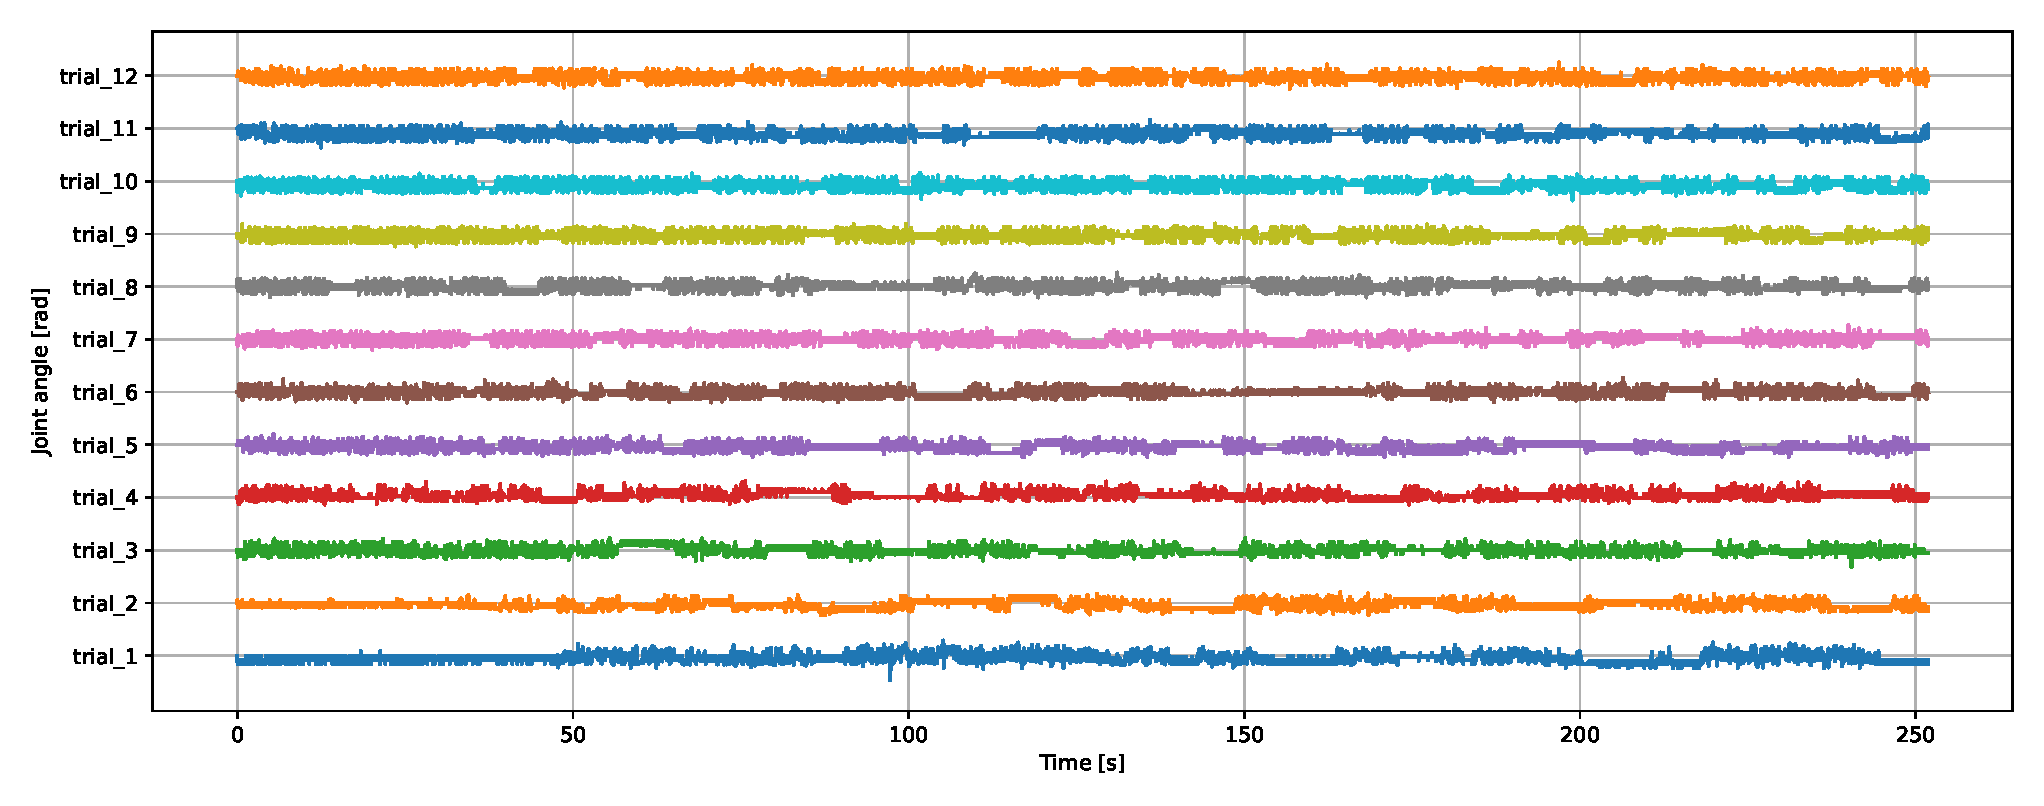
\includegraphics[width=\textwidth]{angle_angle_LH_leg_Coxa_yaw}
			\caption{left hind Coxa yaw angle}
			\label{fig::lh_coxa_yaw}
		\end{center}
	\end{subfigure}
	
	\begin{subfigure}[h]{0.6\textwidth}
		\begin{center}
			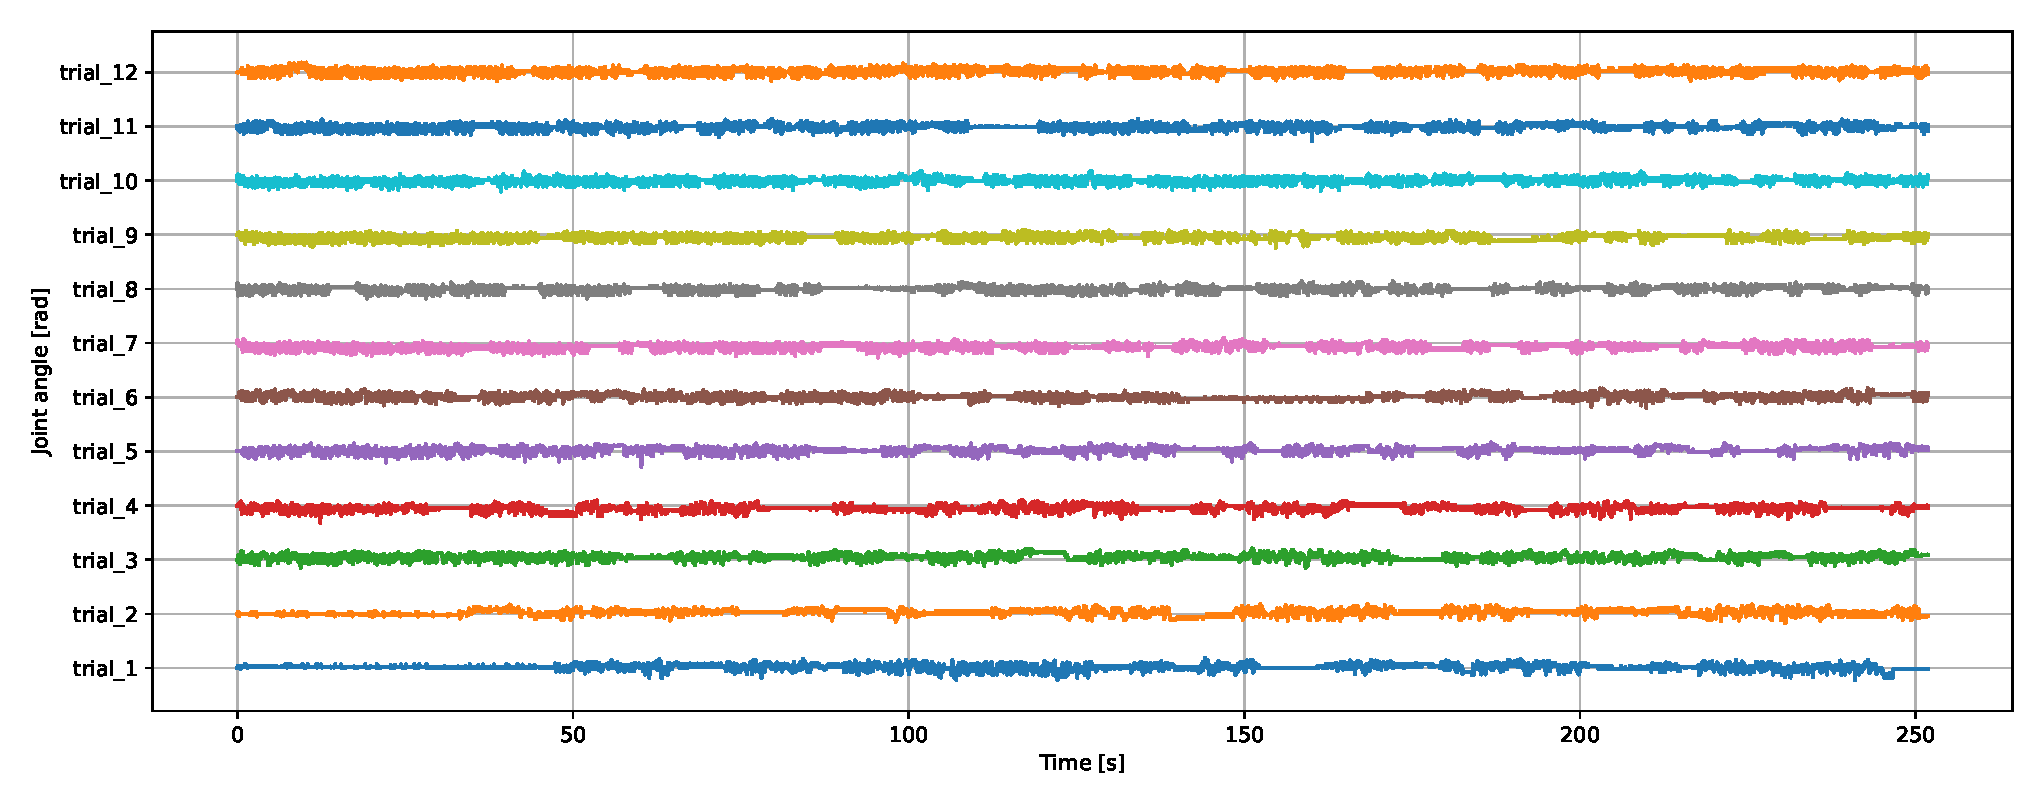
\includegraphics[width=\textwidth]{angle_angle_RF_leg_Coxa_yaw}
			\caption{right front Coxa yaw angle}
		\end{center}
	\end{subfigure}
	
	\begin{subfigure}[h]{0.6\textwidth}
		\begin{center}
			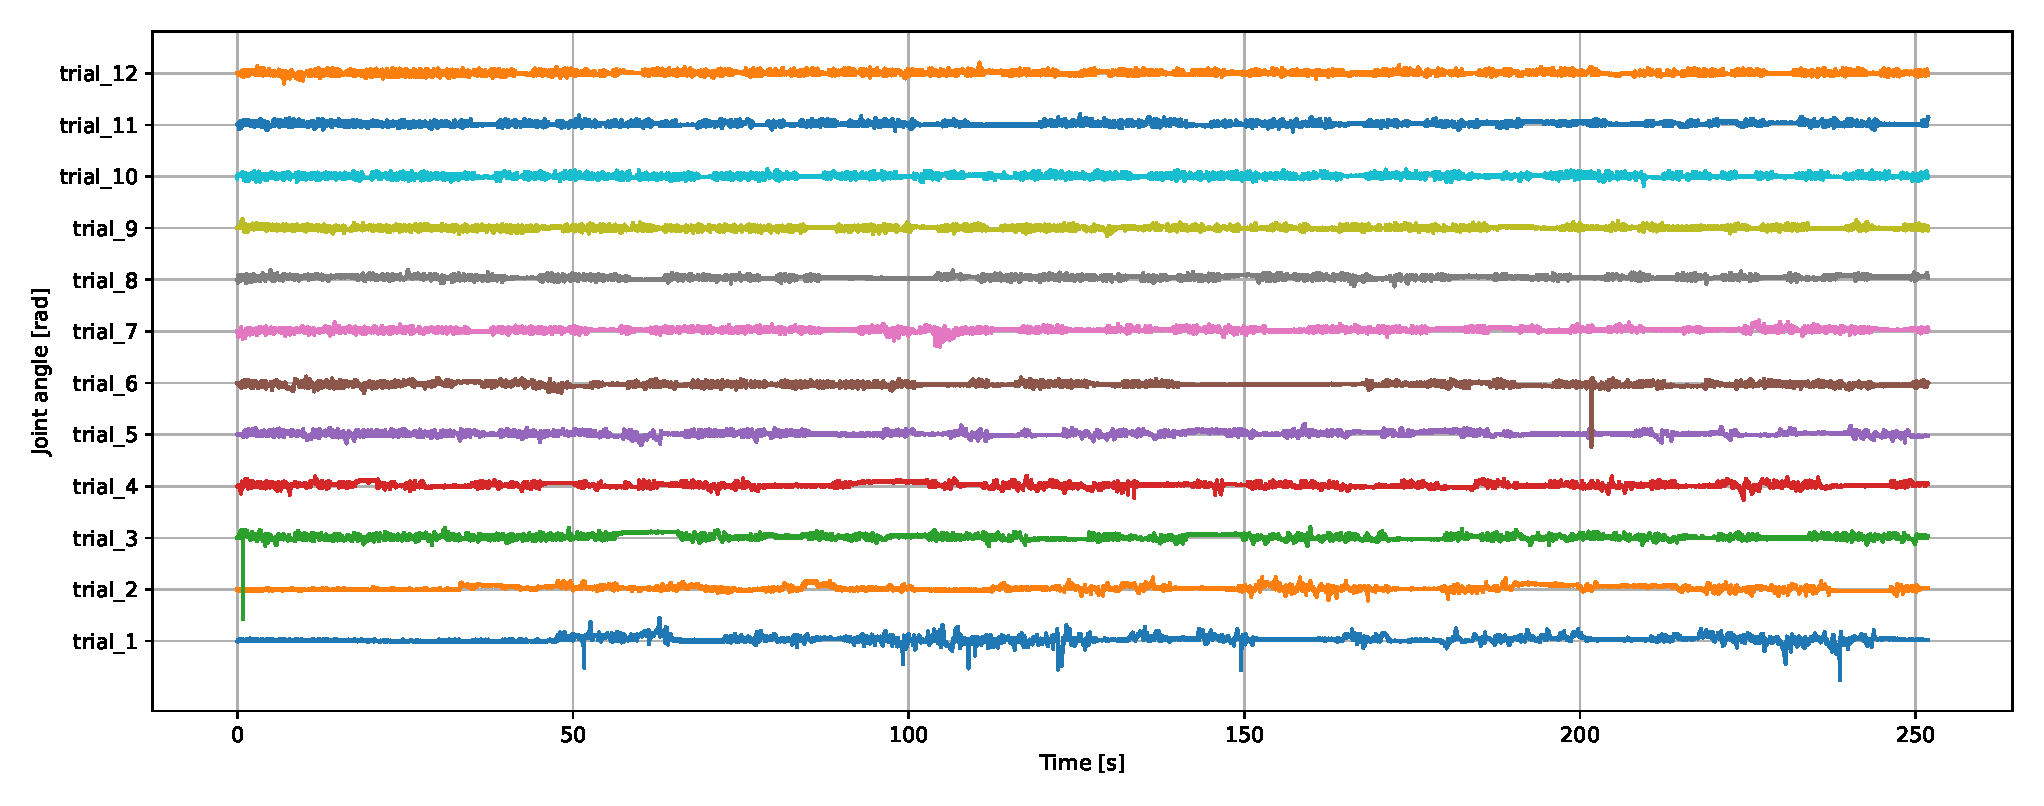
\includegraphics[width=\textwidth]{angle_angle_RH_leg_Coxa_roll}
			\caption{right hind Coxa roll angle}
		\end{center}
	\end{subfigure}
	\caption{A few joint angle signals as provided in the data set.}
	\label{fig::joint_angle}
\end{figure}

\begin{figure}[H]
	\begin{subfigure}[h]{0.6\textwidth}
		\begin{center}
			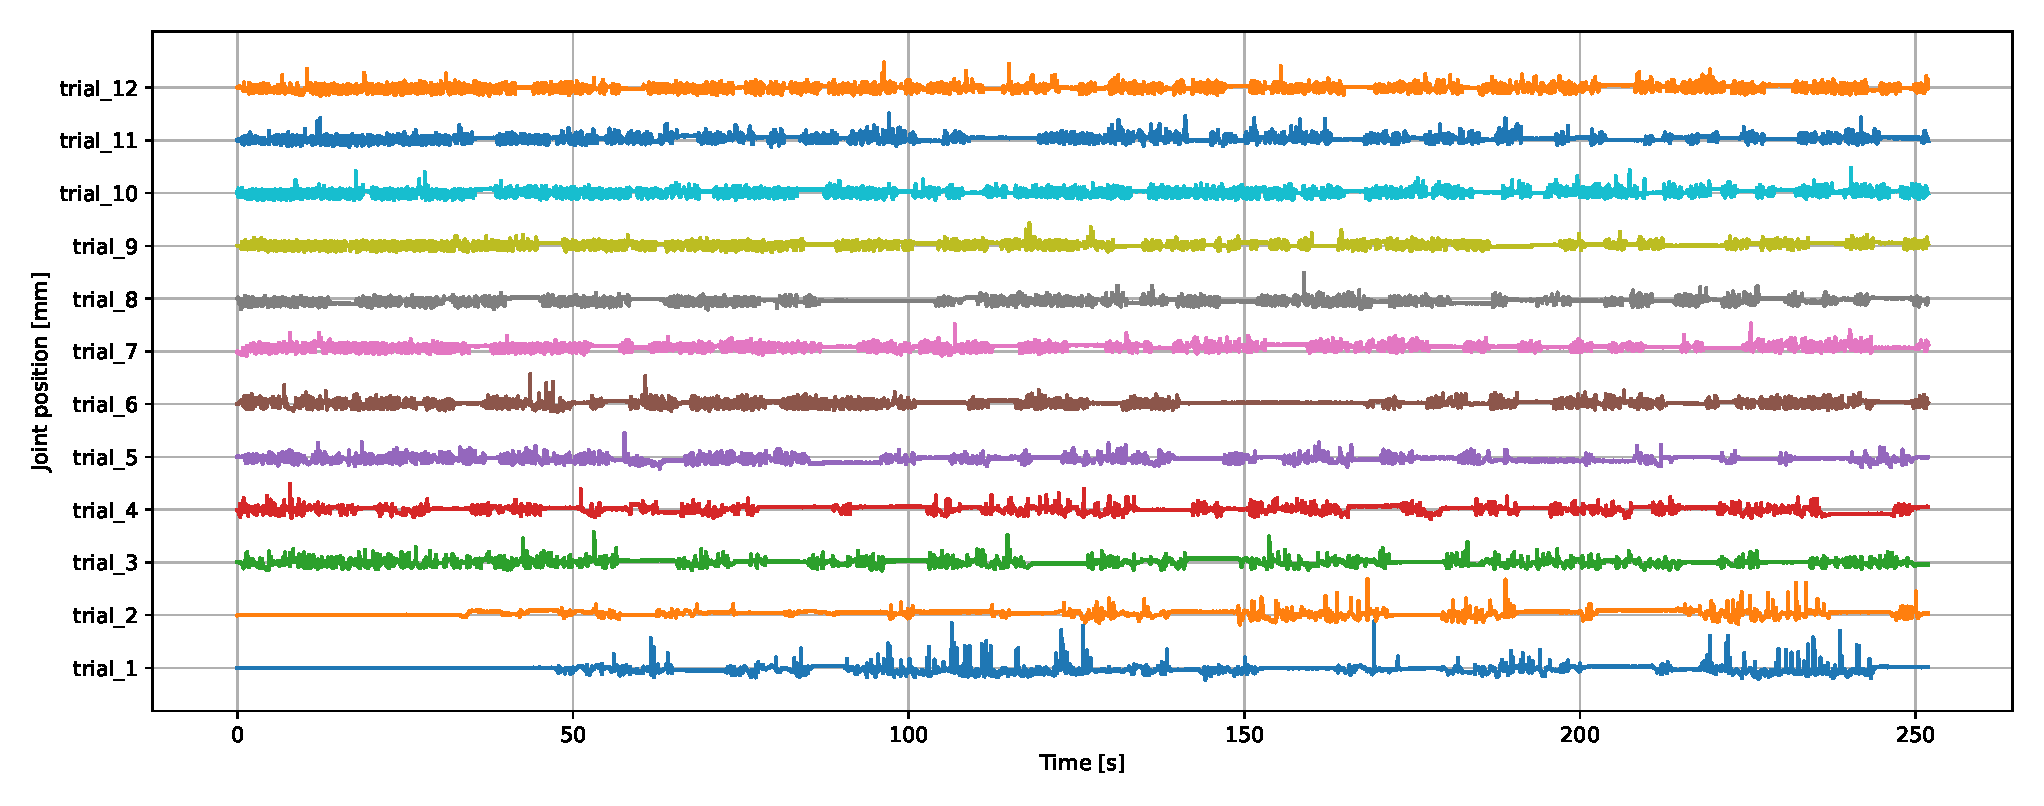
\includegraphics[width=\textwidth]{position_joint_LH_leg_Claw_z}
			\caption{left hind Claw $z$ position}
			\label{fig::lh_claw_z}
		\end{center}
	\end{subfigure}
	
	\begin{subfigure}[h]{0.6\textwidth}
		\begin{center}
			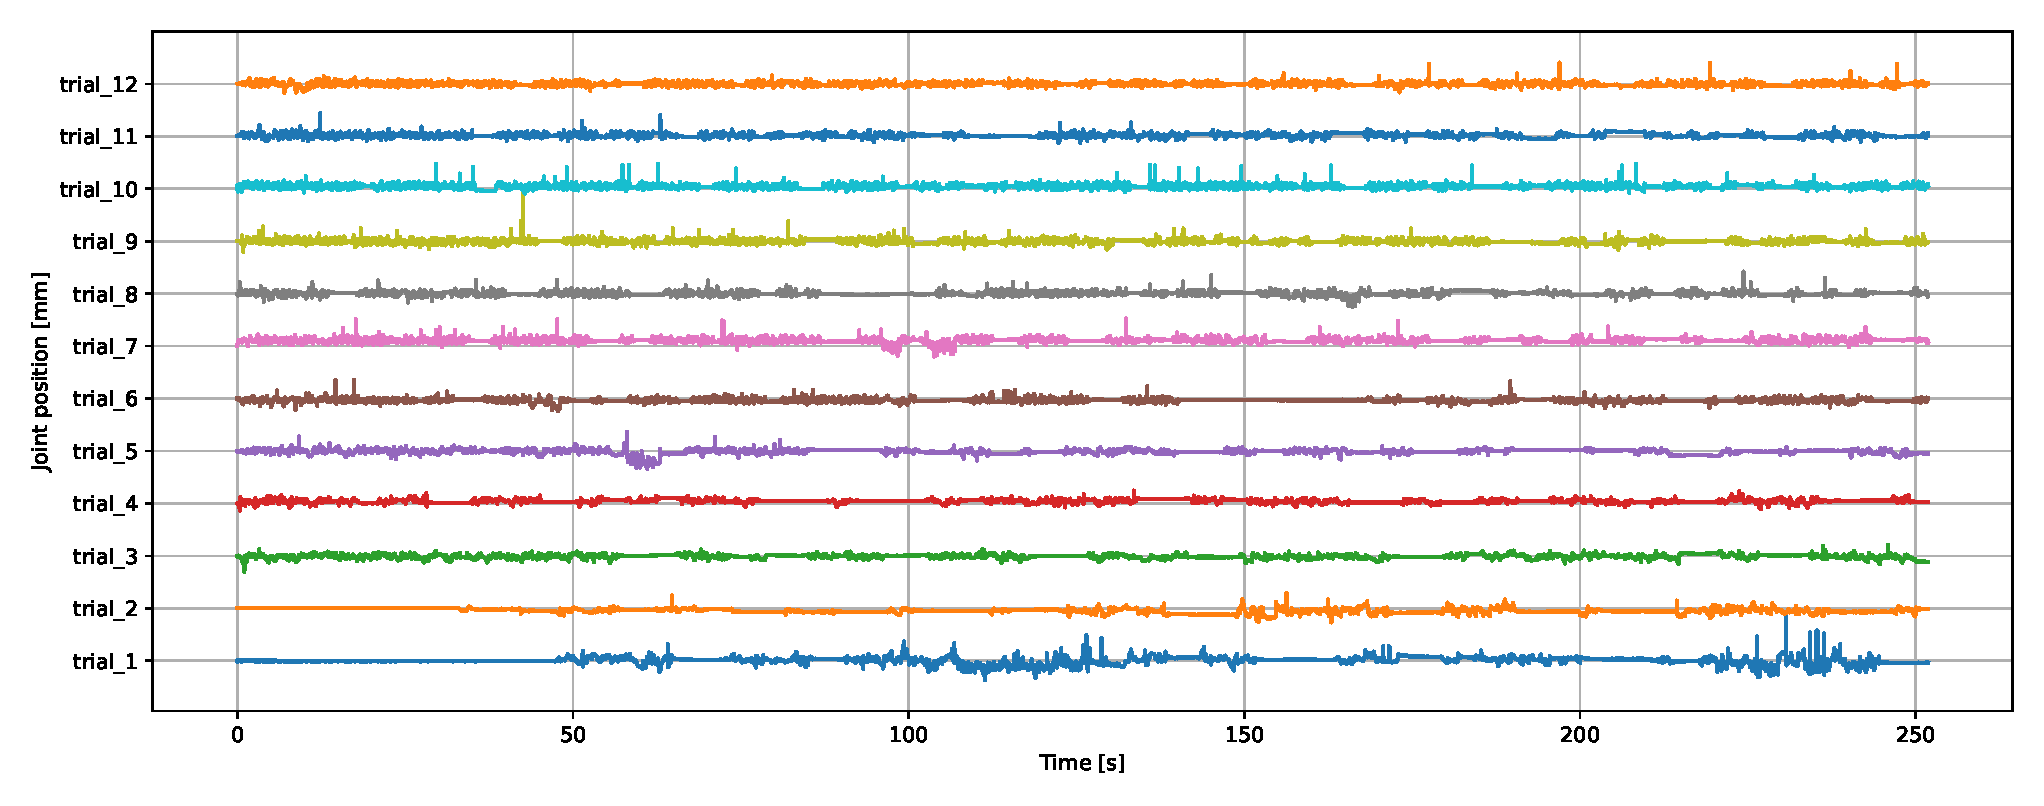
\includegraphics[width=\textwidth]{position_joint_LH_leg_Tarsus_y}
			\caption{left hind Tarsus $y$ position}
			\label{fig::lh_tarsus_y}
		\end{center}
	\end{subfigure}
	
	\begin{subfigure}[h]{0.6\textwidth}
		\begin{center}
			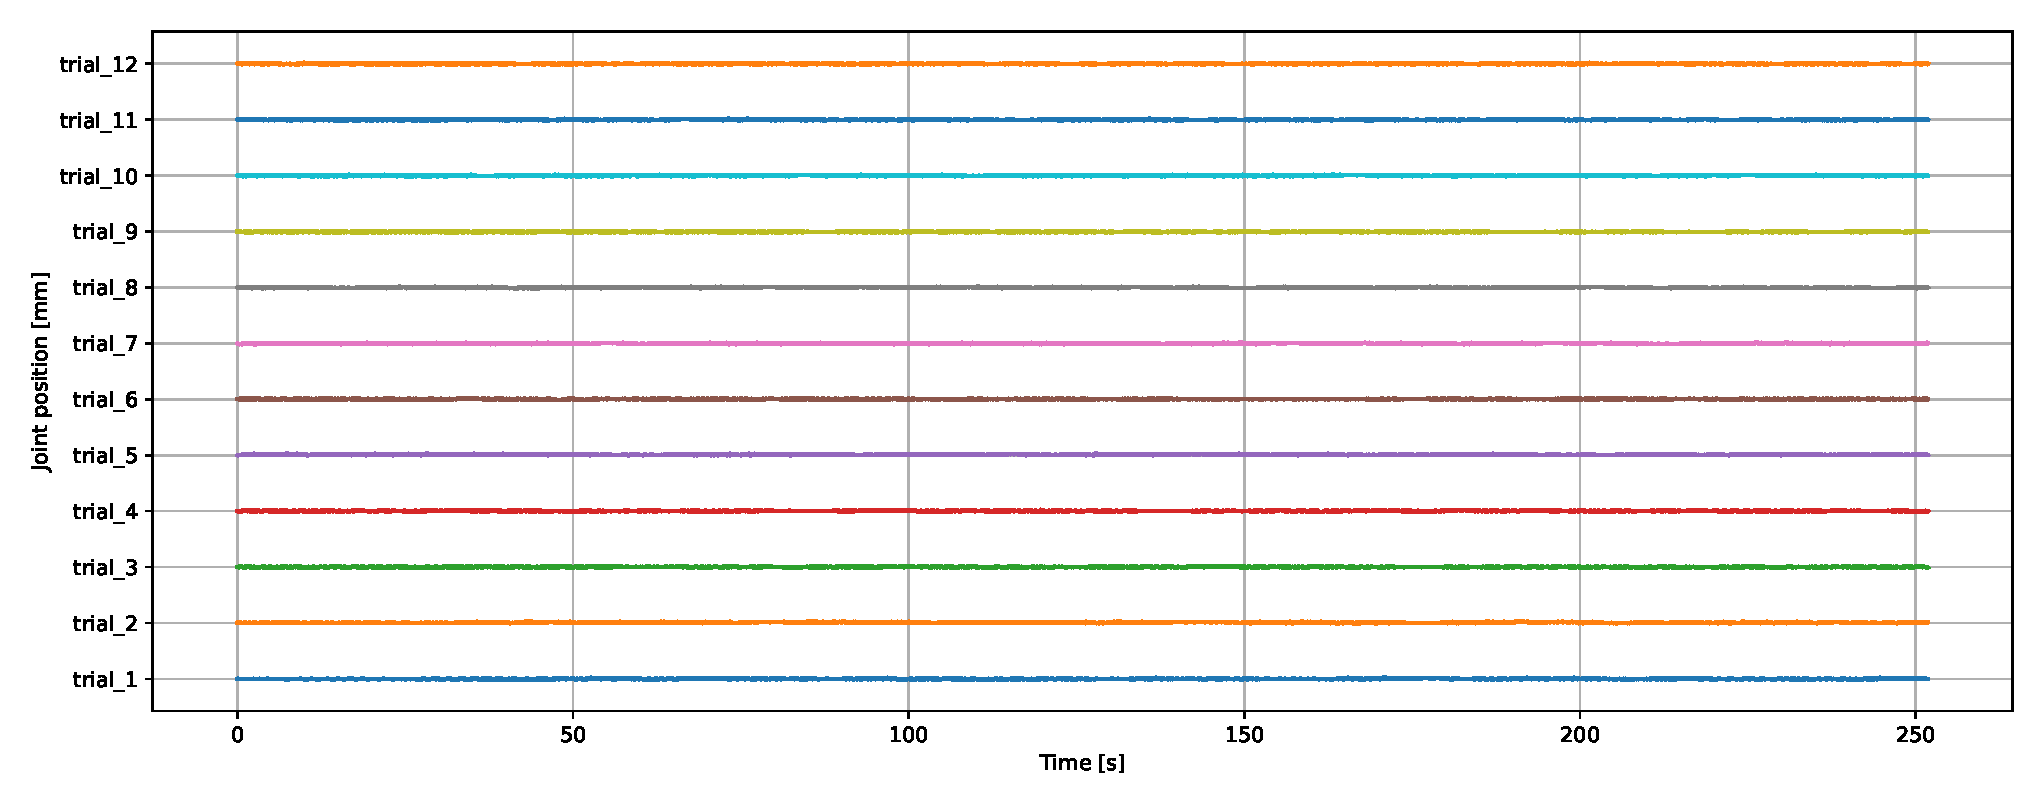
\includegraphics[width=\textwidth]{position_joint_RF_leg_Coxa_z}
			\caption{right front Coxa $z$ position}
			\label{fig::rf_coxa_z}
		\end{center}
	\end{subfigure}
	\caption{A few joint position signals as provided in the data set.}
	\label{fig::joint_position}
\end{figure}

We can see that some segments, within specifics degree of freedoms, are consistently immobile across the trials, like the right front Coxa $z$ position,~\ref{fig::rf_coxa_z}; while some are consistently mobile, like the left hind Coxa yaw angle (\ref{fig::lh_coxa_yaw}) or the left hind Tarsus $y$ position (\ref{fig::lh_tarsus_y}).

The signals do not display easily recognizable or repetitive patterns across the trials, which makes sense since they depend on the fly's behavior during the trial.

The joint angle data provides good behavioral characterization because they are a relative measure with respect to the fly's leg segments, and so will be really useful for the subsequent analysis.
The joint positions are also helpful but they give less insight, since similar behavior can results in different values, because of the absolute nature of the joint position signal with respect to the fly's leg segments.

\subsection{Neural data}

Neural data was recorded at \SI{16}{\hertz} using two-photon imaging, and was provided as 123 neural signal for all 12 trials.
Because two-photon imaging depends on relative change of fluorescence, the signals require to be normalized.
For that, a baseline was determined and subtracted.
Here it was computed as the minimum of a moving average of the signal over 10 frames for each neuron and each trial.
It makes sense to have independent baselines across neurons and trials, because the hypothesis is that the trials and neurons \textit{recordings} are independent.

\vspace{\baselineskip}

On Figure~\ref{fig::neural_before} below, we can observe a few examples of the neural signals:

\begin{figure}[H]
	\begin{subfigure}[h]{0.6\textwidth}
		\begin{center}
			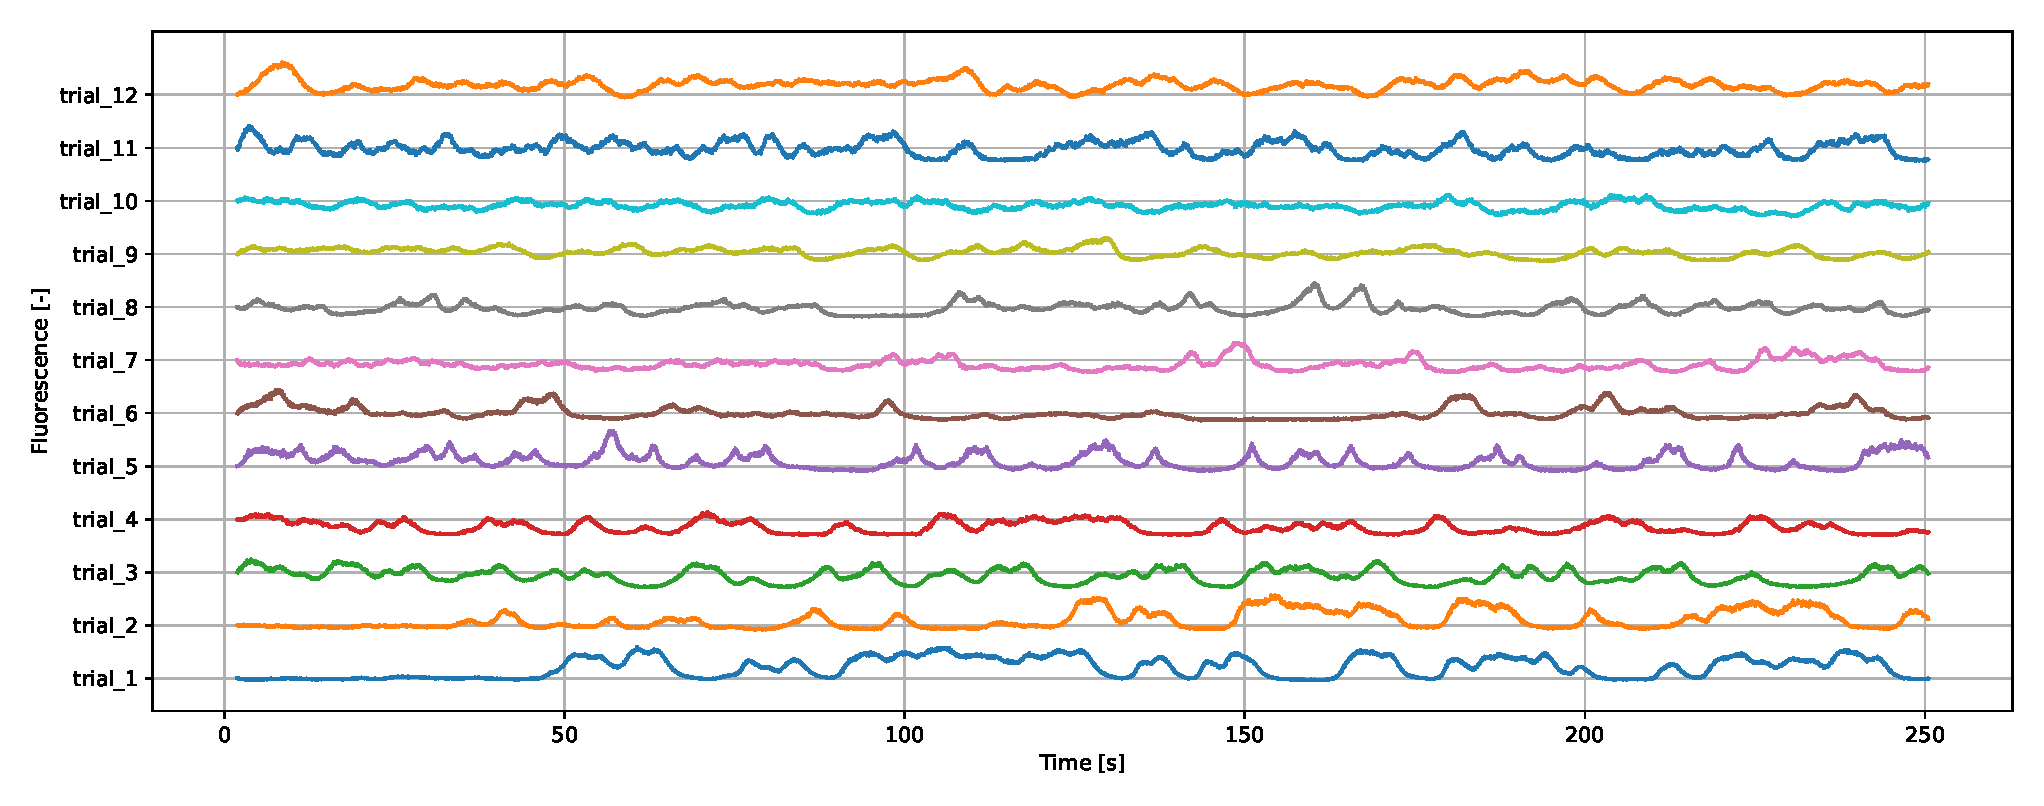
\includegraphics[width=\textwidth]{fluorescence2}
			\caption{neuron 2}
		\end{center}
	\end{subfigure}
	
	\begin{subfigure}[h]{0.6\textwidth}
		\begin{center}
			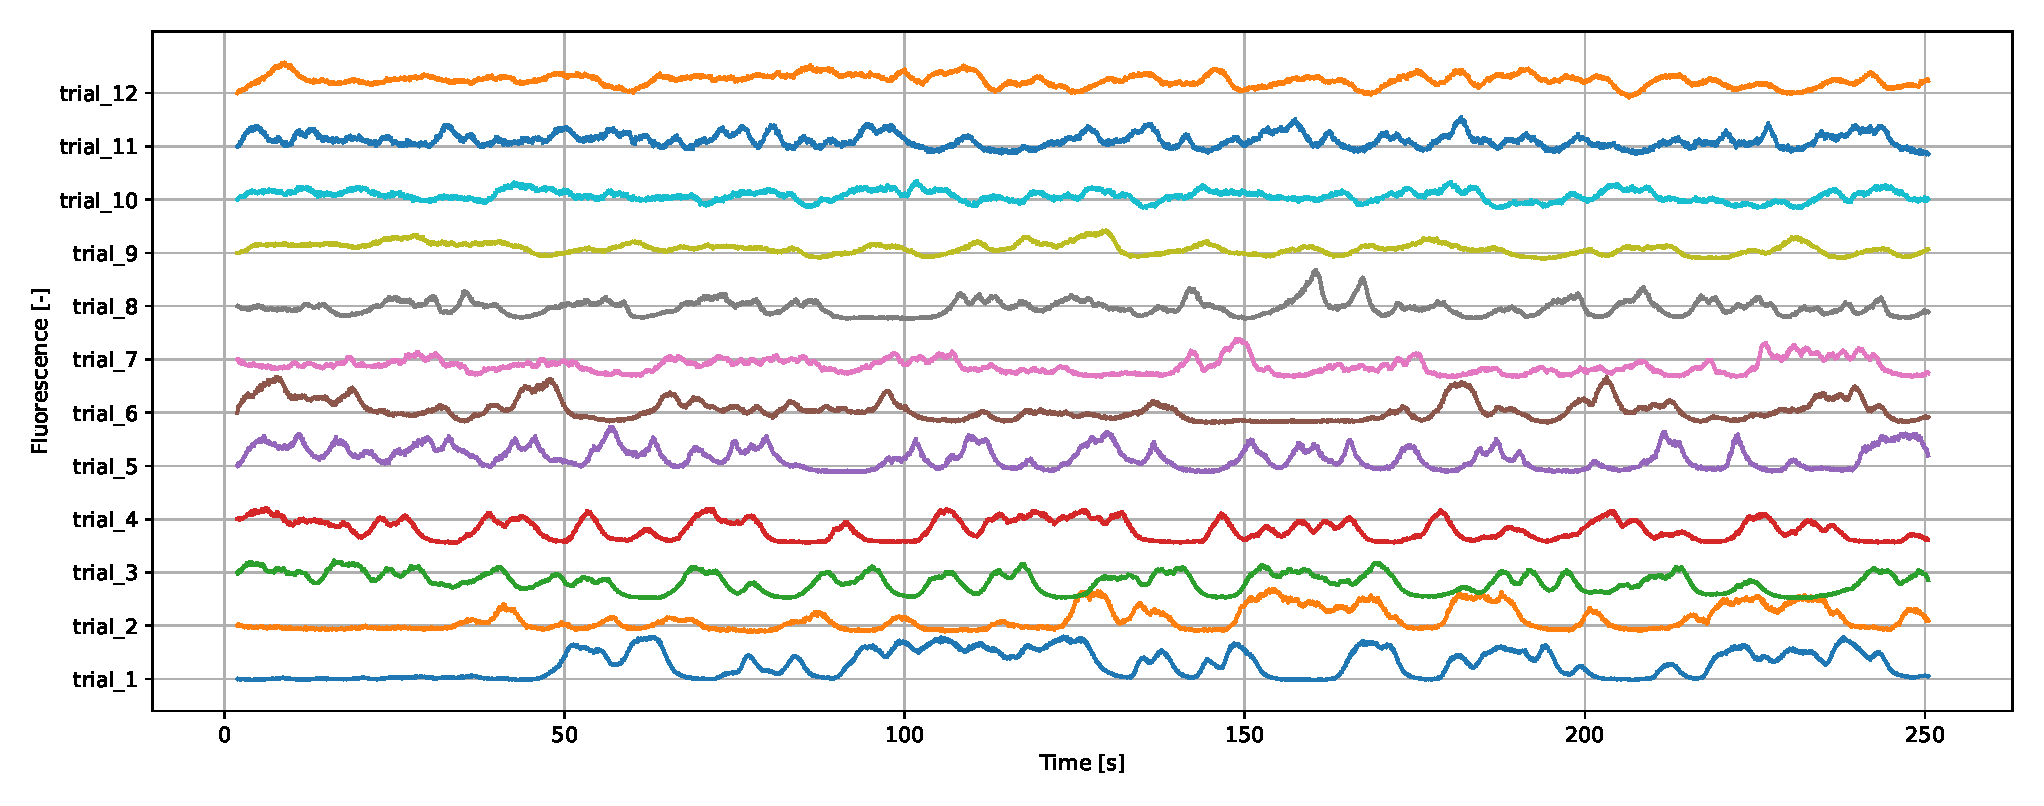
\includegraphics[width=\textwidth]{fluorescence7}
			\caption{neuron 7}
		\end{center}
	\end{subfigure}
	
	\begin{subfigure}[h]{0.6\textwidth}
		\begin{center}
			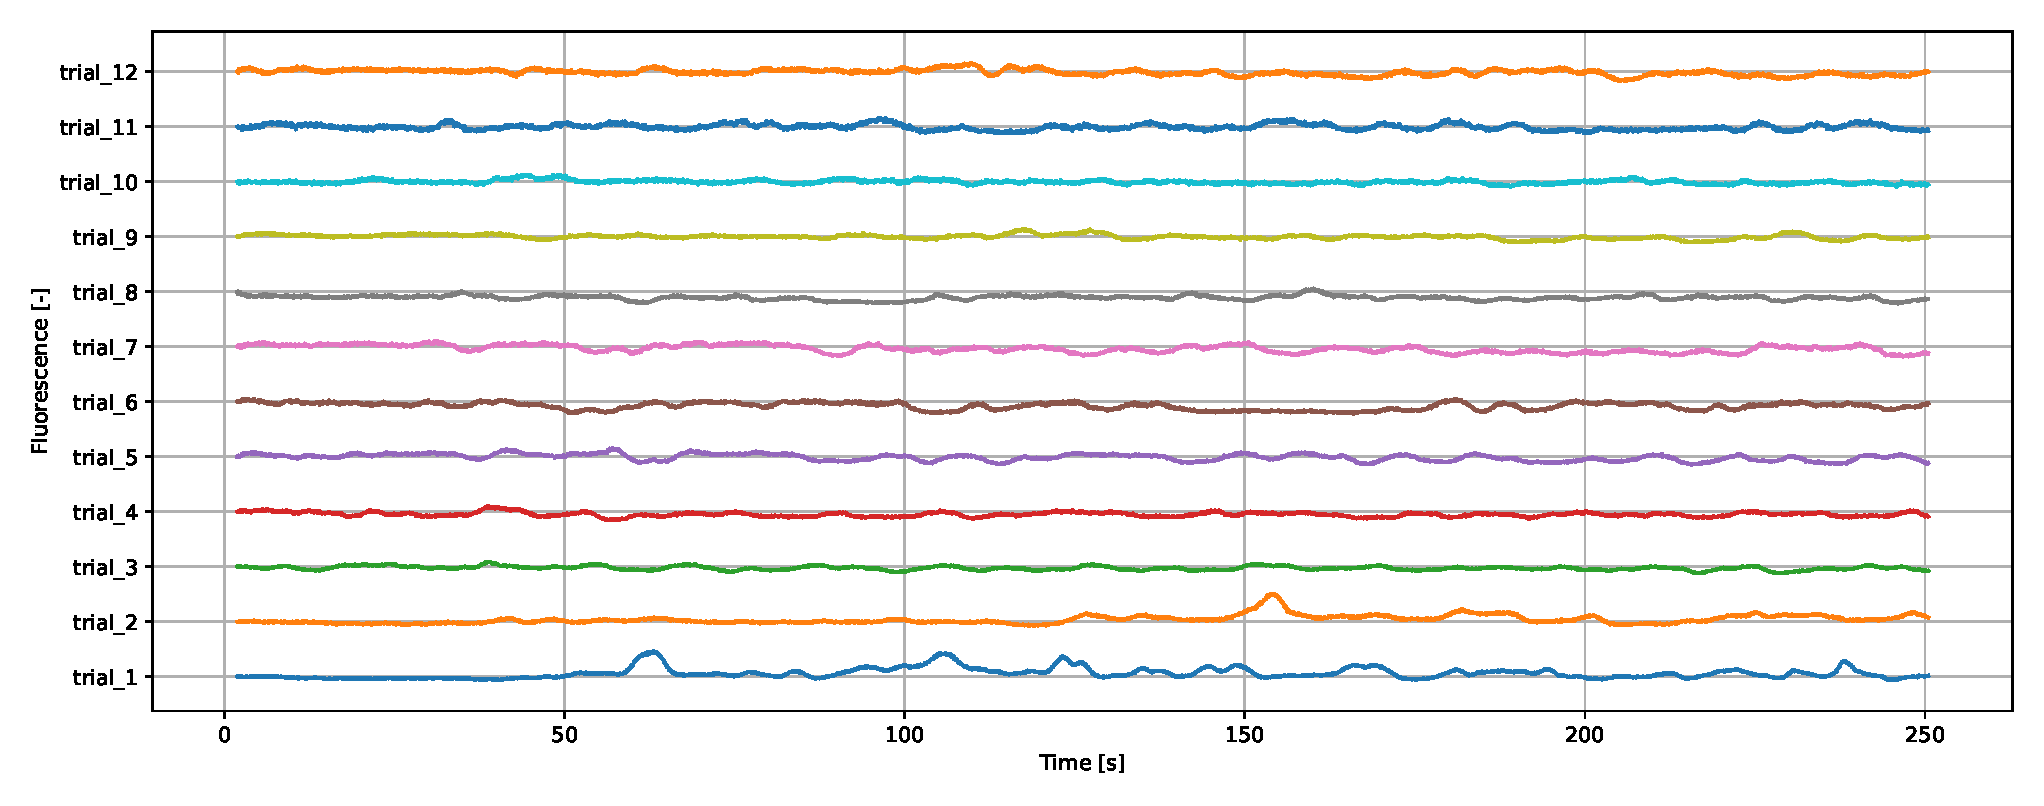
\includegraphics[width=\textwidth]{fluorescence42}
			\caption{neuron 42}
		\end{center}
	\end{subfigure}
	\caption{Neural signals after baseline subtraction (two-photon imaging produces data with an arbitrary unit).}
	\label{fig::neural_before}
\end{figure}

As can be seen on Figure~\ref{fig::neural_before}, the neural signals are quite noisy, and require low-pass filtering.
The noise is typical of in vivo recordings, and is mainly due to small voltage fluctuations in the neuron membrane as well as noise from the recording process. 

\begin{figure}[H]
	\begin{center}
		\includesvg[width=0.5\textwidth]{noise}
	\end{center}
	\caption{Window of neural fluorescence with different filters applied for noise reduction assessment.}
	\label{fig::neural_denoizing}
\end{figure}

On Figure~\ref{fig::neural_denoizing}, we can see that a Gaussian filter with $\sigma=6$ is appropriate to reduce the noise in a satisfactory manner.

\vspace{\baselineskip}

A few samples of the neural data after noise reduction are displayed on Figure~\ref{fig::neural_after} below:

\begin{figure}[H]
	\begin{subfigure}[h]{0.6\textwidth}
		\begin{center}
			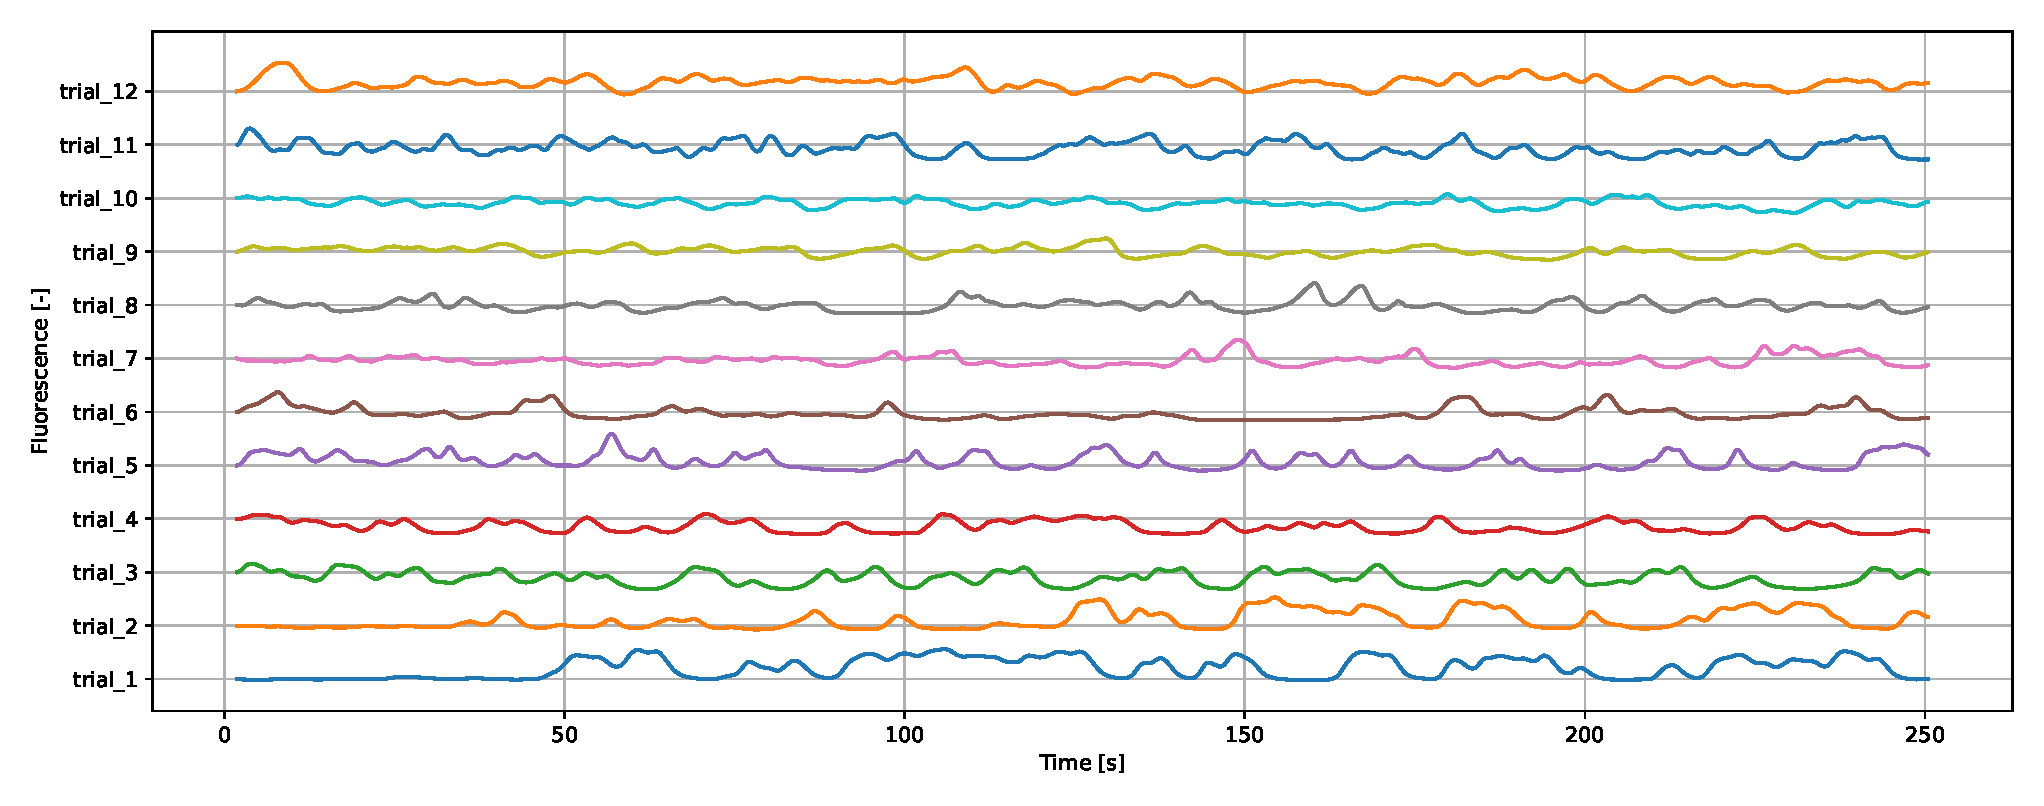
\includegraphics[width=\textwidth]{fluorescence_denoized2}
			\caption{neuron 2}
		\end{center}
	\end{subfigure}
	
	\begin{subfigure}[h]{0.6\textwidth}
		\begin{center}
			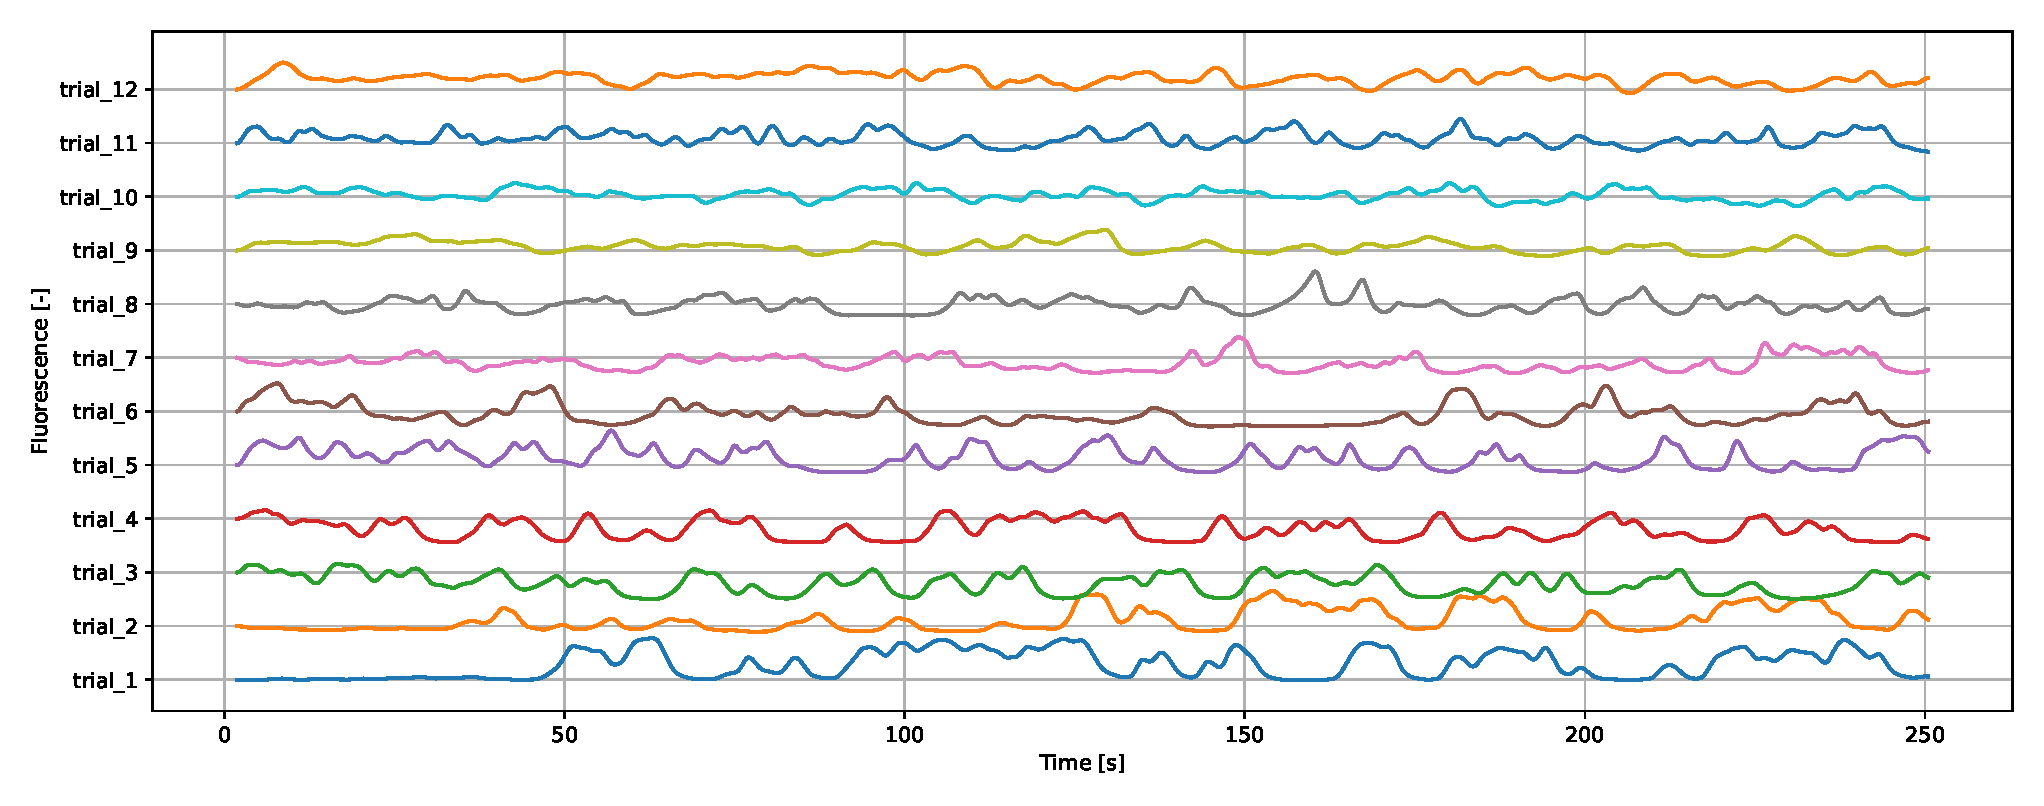
\includegraphics[width=\textwidth]{fluorescence_denoized7}
			\caption{neuron 7}
		\end{center}
	\end{subfigure}
	
	\begin{subfigure}[h]{0.6\textwidth}
		\begin{center}
			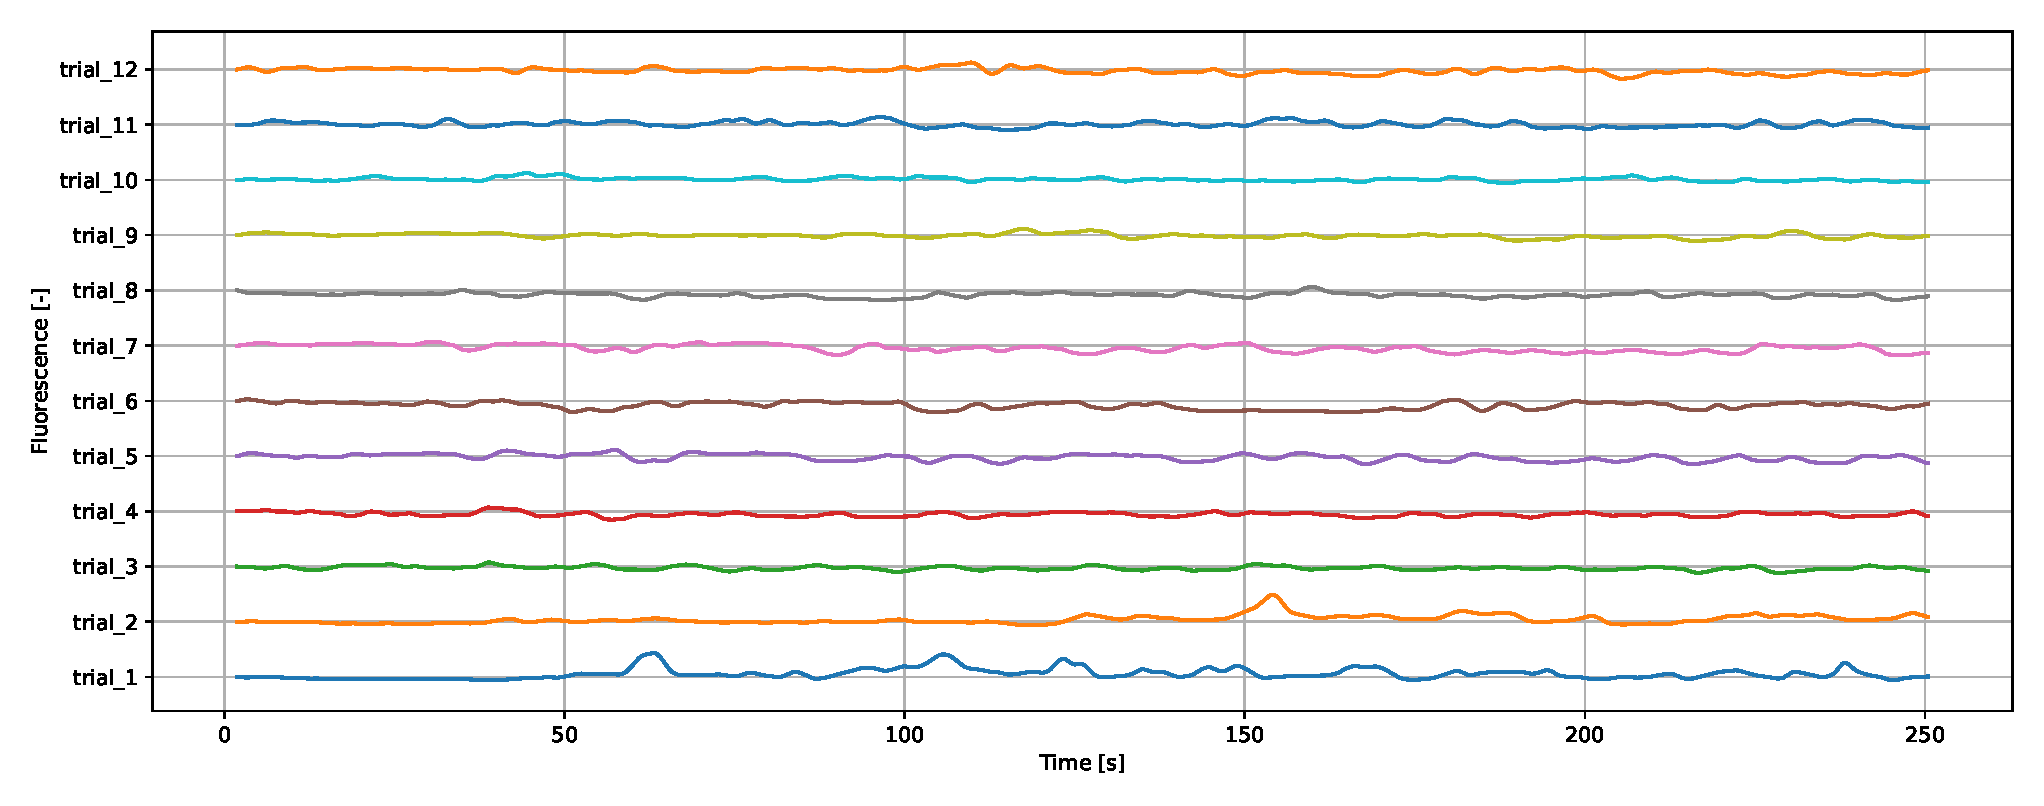
\includegraphics[width=\textwidth]{fluorescence_denoized42}
			\caption{neuron 42}
		\end{center}
	\end{subfigure}
	\caption{Neural signals after noise reduction (two-photon imaging produces data with an arbitrary unit).}
	\label{fig::neural_after}
\end{figure}

They are the same neurons as on Figure~\ref{fig::neural_before}, and when comparing both, it is visible that the noise reduction is satisfactory: most of the information is kept, while most of the noise is removed.

From these signals, the main observation is that some neurons are much more active than others, some trials displays more activity than other, and that the signals exhibit varied values.
This is consistent with the fact that the data is observational, and the flies are free to behave on the air-suspended spherical treadmill.

\vspace{\baselineskip}

After this preprocessing, the neural data is ready to be used.

\newpage

	\section{Data dimensionality reduction and visualization}

After preprocessing, our data was further manipulated in order to reduce its dimensionality.
This allows observation of the data into lower dimensions and gaining insight on how the data is organized, and whether it is linked in meaningful ways~\cite{cunningham2014},~\cite{valletta2017}.
Reducing the dimensionality also allows to plot the data in graphs that are visually meaningful, since after the third dimension, this becomes increasingly difficult.

\subsection{Behavioral data}

Because the goal of the project is to understand the relationship between the DNs of \textit{Drosophila} and its behavior, the behavioral and neural data must be formatted to allow for comparison.
In the case of the behavioral data, which was recorded at \SI{100}{\hertz}, it means downsampling the data to match the \SI{16}{\hertz} of the neural data.
In the downsampled dataset, the distinction between the predicted and manually labeled categorical value for the behavioral classes was merged altogether, with only one label per sample (instead of two, one predicted, one manual).
That label is based on both the predicted and manually labeled values, by considering the most prevalent categorical behavior within the time frame considered for the downsampling.
Indeed, the manual labeling done previously on the initial dataset had proven that the predictions were quite bad: in the original behavioral dataset, there is 22\% of mismatch between the manual labels (67430 mismatches for 302400 total samples), which are summarized in Table~\ref{tab::behavioral_data_count}.

\begin{table}[htbp]
	\sffamily
	\arrayrulecolor{white}
	\arrayrulewidth=1pt
	\renewcommand{\arraystretch}{1.5}
	\rowcolors[\hline]{1}{.!50!White}{}
	\centering
	\begin{tabular}{@{} A|A|B @{}}
		\cellcolor{ForestGreen}\arraycolor{White}\bfseries Behavior prediction &
		\cellcolor{ForestGreen}\arraycolor{White}\bfseries Manual behavior labeling &
		\cellcolor{ForestGreen}\arraycolor{White}\bfseries Count \\   
		\arraycolor{Black}
		Resting & Walking & 13645 \\
		Resting & Anterior grooming & 12745 \\
		Walking & Anterior grooming & 12020 \\
		Walking & Resting & 10641 \\
		Resting & Abdominal pushing & 4156 \\
		Front leg Grooming & anterior grooming & 4143 \\
		Walking & Abdominal pushing & 2806 \\
		Front leg grooming & Walking & 1730 \\
		Antennal grooming & Anterior grooming & 1390 \\
		Walking & Posterior grooming & 1109 \\
		Front leg grooming & Resting & 866 \\
		Resting & Posterior grooming & 835 \\
		Abdominal grooming & Abdominal pushing & 455 \\
		Abdominal grooming & Resting & 164 \\
		Front leg grooming & Posterior grooming & 111 \\
		Antennal grooming & Walking & 108 \\
		Eye grooming & Anterior grooming & 103 \\
		Hind leg grooming & Abdominal pushing & 102 \\
		Abdominal grooming & Walking & 75 \\
		Abdominal grooming & Posterior grooming & 49 \\
		Hind leg grooming & Walking & 32 \\
		Antennal grooming & Posterior grooming & 31 \\
		Antennal grooming & Resting & 22 \\
		Hind leg grooming & Posterior grooming & 16 \\
		Front leg grooming & Abdominal pushing & 12 \\
		Eye grooming & Resting & 9 \\
		Hind leg grooming & Resting & 9 \\
		Eye grooming & Walking & 6 \\
		Antennal grooming & Abdominal pushing & 5 \\
		Eye grooming & Posterior grooming & 4 \\
		Abdominal grooming & Anterior grooming & 0 \\
	\end{tabular}
	\caption{Differences between behavioral predictions and manual labeling.}
	\label{tab::behavioral_data_count}
\end{table}

\vspace{\baselineskip}

This downsampling led to a reduced behavioral dataset comprised of nine categorical values, summarized in Table~\ref{tab::behavioral_data_length}.
Notably, the eye grooming label disappeared (it was only predicted a few times, but not witnessed during the manual labeling), while some new behaviors not manually labeled were introduced, coming from the predicted behaviors.

\begin{table}[htbp]
	\sffamily
	\arrayrulecolor{white}
	\arrayrulewidth=1pt
	\renewcommand{\arraystretch}{1.5}
	\rowcolors[\hline]{1}{.!50!White}{}
	\centering
	\begin{tabular}{@{} A|B @{}}
		\cellcolor{ForestGreen}\arraycolor{White}\bfseries Behavior &
		\cellcolor{ForestGreen}\arraycolor{White}\bfseries Length \\   
		\arraycolor{Black}
		Walking 			& 23228 \\
		Resting 			& 18834 \\
		Anterior grooming 	& 4412 	\\
		Abdominal pushing 	& 1157 	\\
		Front leg grooming 	& 321 	\\
		Posterior grooming 	& 304 	\\
		Antennal grooming 	& 165 	\\
		Abdominal grooming 	& 57 	\\
		Hind leg grooming 	& 2 
	\end{tabular}
	\caption{Categorical values in the reduced behavioral dataset.}
	\label{tab::behavioral_data_length}
\end{table}

\subsection{Kinematic data}

Both the kinematic data and the neural data contain a lot of information.
The kinematic data alone describes 132 temporal variables, at \SI{100}{\hertz} for $\sim\SI{250}{\second}$ over twelve trials.
In order not to fall prey to the curse of dimensionality and sparsity which follows, the kinematic data was projected through a Principal Component Analysis (PCA).
A PCA projects $n$ samples of $p$-dimensional data in an orthogonal, also $p$-dimensional space, the trick being that the destination space, which dimensions are called principal components, are ordered by variance of the data explained and computed so that each successive one explains the most variance possible.
Thus, the higher dimensions of the projected space explain the most variance, while the last explain the least variance.
If the data is entirely uncorrelated, a PCA should explain approximately the same amount of variance per principal component, while a highly correlated dataset will have most of its variance explained by the first principal components.

\vspace{\baselineskip}

Here, the kinematic dataset was separated between the joint angles and the joint positions, and then a PCA was ran on each trial.
Thus, there was a total of 24 PCA.
For the joint positions, the $p$ dimensions of the dataset are the 90 temporal joint position variables, while each temporal point is a sample.
For the joint angles, the $p$ features are the 42 temporal joint angle variables.

\vspace{\baselineskip}

After the PCA, we applied a wavelet transform to analyze the dynamics of the fly's joints.
We used the normalized Morlet wavelet transform from the \verb*|behavelet| package \cite{berman2014}, which analyses the frequency components of the leg segments movements across time.
The Morlet wavelet is composed of a complex exponential multiplied by a Gaussian window, which allows the detection of short oscillations in the time domain.
The Morlet wavelet was applied to the output of the PCA.

\vspace{\baselineskip}

In order to have different visualizations of the dataset, we also applied a t-distributed Stochastic Neighbor Embedding (t-SNE).
Contrary to a PCA, a t-SNE is a non linear method.
It finds mapping of the data points which preserve local neighborhood by first constructing a probability distribution over pairs of similar high-dimensional data points.
Then it defines a similar probability distribution in the low-dimensional map and minimize the Kullback-Leibler (KL) divergence between the two distributions.
The KL divergence is a measure of the difference between the probability distributions.
The t-SNE was applied both directly after the PCAs, and after the wavelet transforms; both for the joint positions and joint angles.
The results are displayed on Figure~\ref{fig::kinematic_data_tsne}.

\begin{figure}[htbp]
	\begin{subfigure}{.49\textwidth}
		\begin{center}
			\includesvg[width=\textwidth]{tsne_joint_pca_s}
			\caption{t-SNE of joint positions from PCA data}
		\end{center}
	\end{subfigure}
	\begin{subfigure}{.49\textwidth}
		\begin{center}
			\includesvg[width=\textwidth]{tsne_joint_wave_s}
			\caption{t-SNE of joint positions from wavelet data}
		\end{center}
	\end{subfigure}
	\begin{subfigure}{.49\textwidth}
		\begin{center}
			\includesvg[width=\textwidth]{tsne_angle_pca_s}
			\caption{t-SNE of joint angles from PCA data}
		\end{center}
	\end{subfigure}
	\begin{subfigure}{.49\textwidth}
		\begin{center}
			\includesvg[width=\textwidth]{tsne_angle_wave_s}
			\caption{t-SNE of joint angles from wavelet data}
		\end{center}
	\end{subfigure}
	\caption{t-SNE plots on the kinematic data after dimensionality reduction.}
	\label{fig::kinematic_data_tsne}
\end{figure}

On Figure~\ref{fig::kinematic_data_tsne}, the data is segregated by behavioral categories.
Unfortunately, it did not produce a meaningful output that would help gain insight on the organization of the kinematic data.

\subsection{Neural data}

\subsubsection{Each neuron a feature, each time point a sample}

We first applied PCA on the neural data with each neuron as a feature and each time point as a sample.
The three first principal components are plotted on Figure~\ref{fig::neural_data_pca1}.

\begin{figure}[htbp]
	\begin{center}
		\begin{subfigure}{\textwidth}
			\begin{center}
				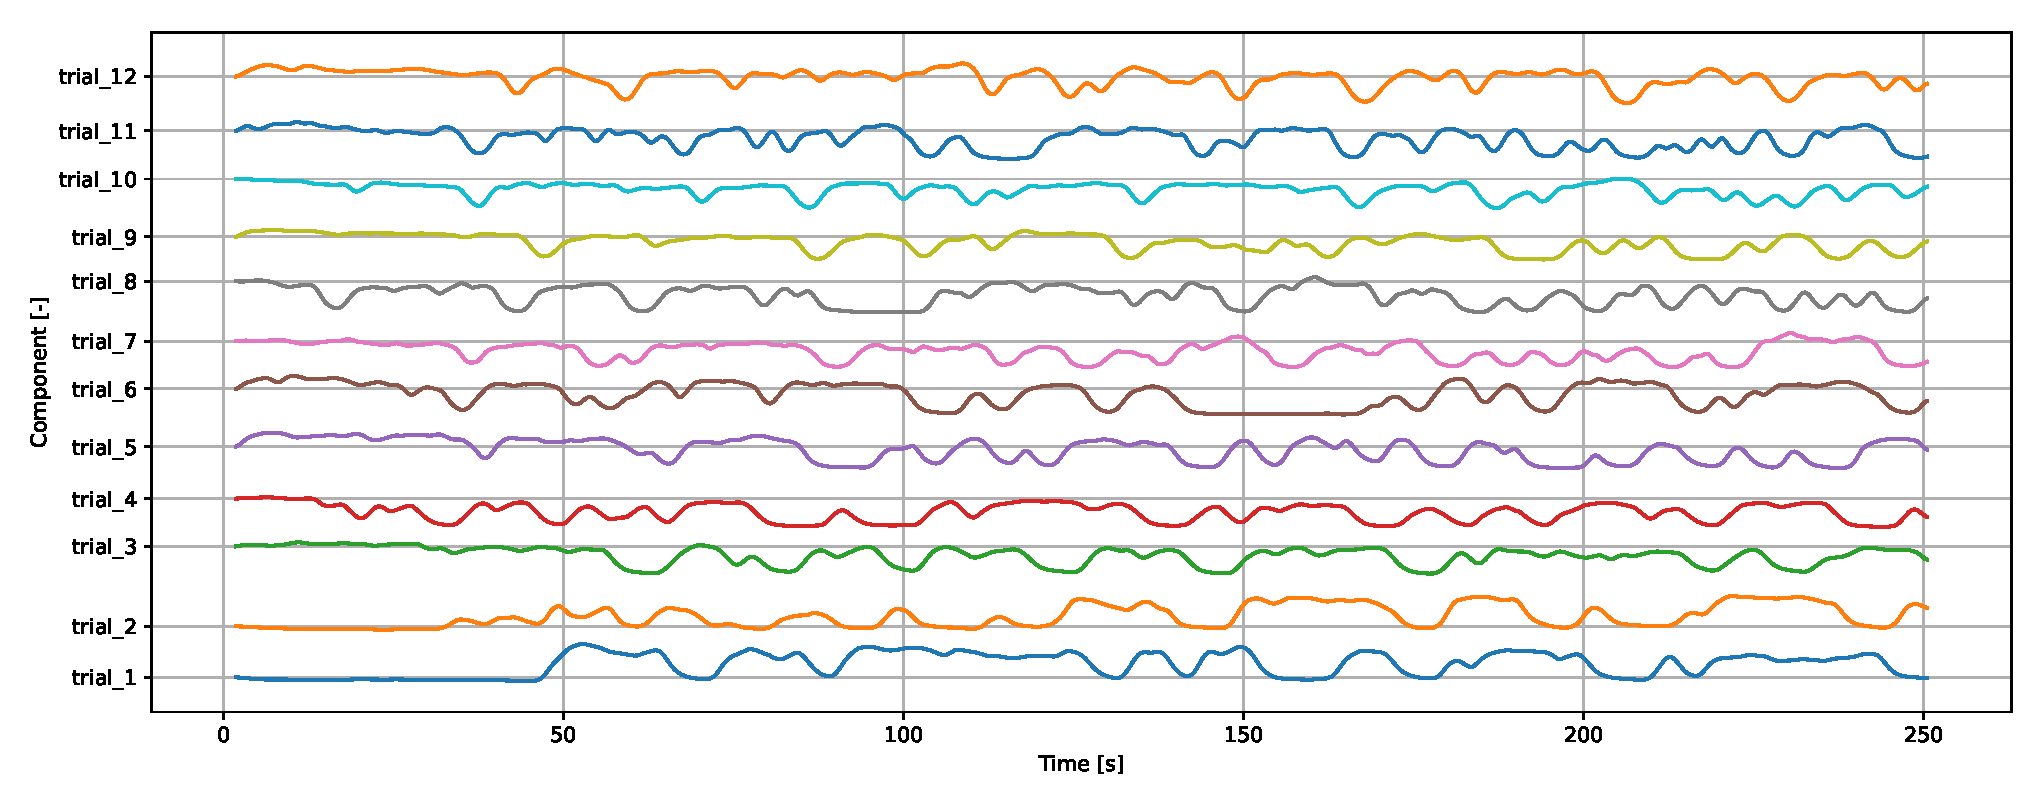
\includegraphics[width=\textwidth]{nd_pca_component_0}
				\caption{Component 0}
			\end{center}
		\end{subfigure}
		\newline
		\begin{subfigure}{\textwidth}
			\begin{center}
				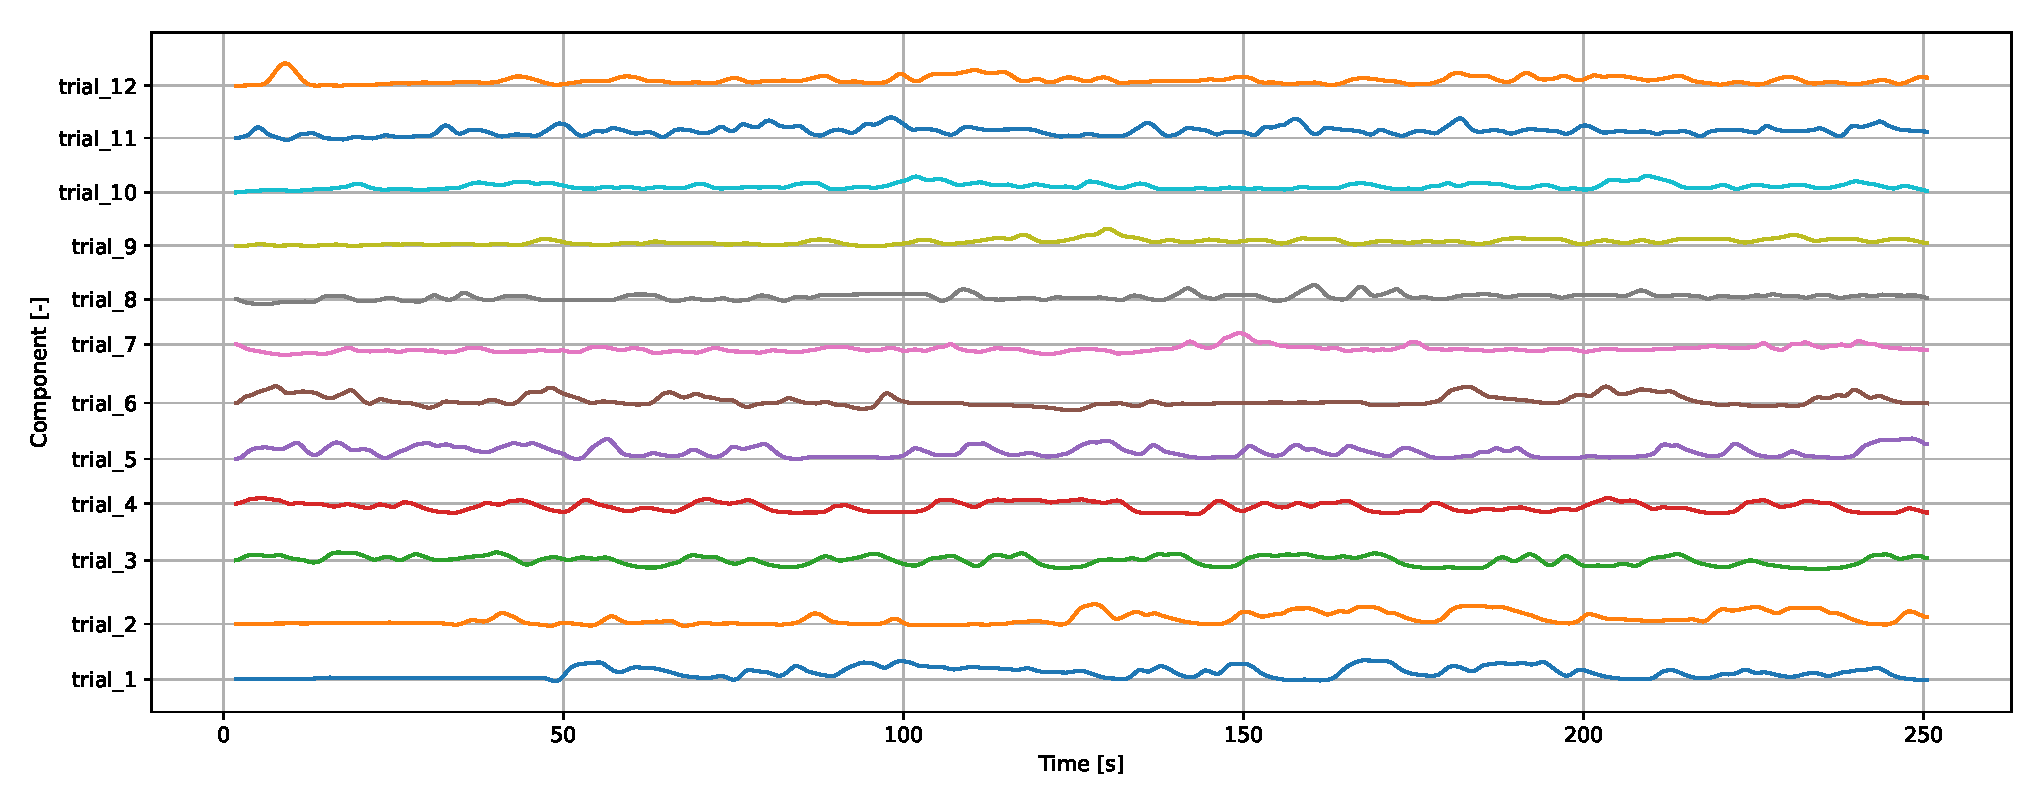
\includegraphics[width=\textwidth]{nd_pca_component_1}
				\caption{Component 1}
			\end{center}
		\end{subfigure}
		\newline
		\begin{subfigure}{\textwidth}
			\begin{center}
				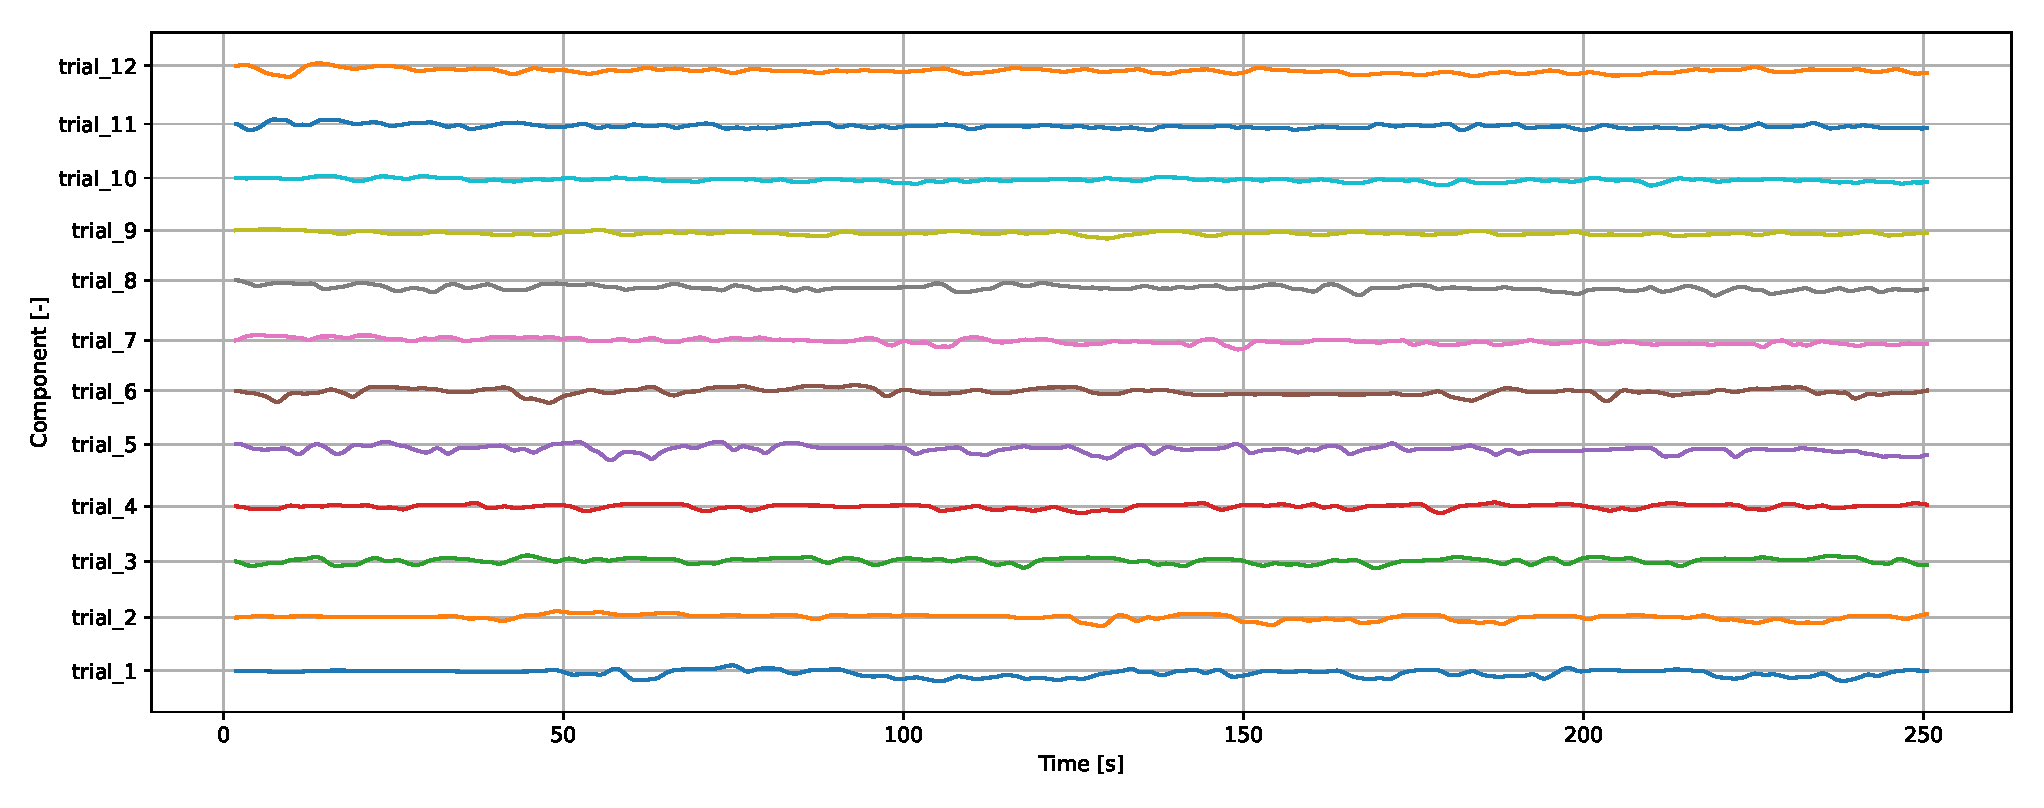
\includegraphics[width=\textwidth]{nd_pca_component_2}
				\caption{Component 2}
			\end{center}
		\end{subfigure}
		\caption{First components of the neural data first PCA (each neuron a feature, each time point a sample).}
		\label{fig::neural_data_pca1}
	\end{center}
\end{figure}

The main observation is that the more we advance in the principal components, the less the signals exhibit variation.
This is due to the fact that PCAs' principal components are specifically constructed to explain the maximum variance in succession.
In this instance, the first 10 components are enough to explain 90\%, as can be seen on Figure~\ref{fig::neural_data_pca1_explained}.
This is quite a low number of components, considering that the initial neural data is composed of 123 dimensions (features).

\begin{figure}[htbp]
	\begin{center}
		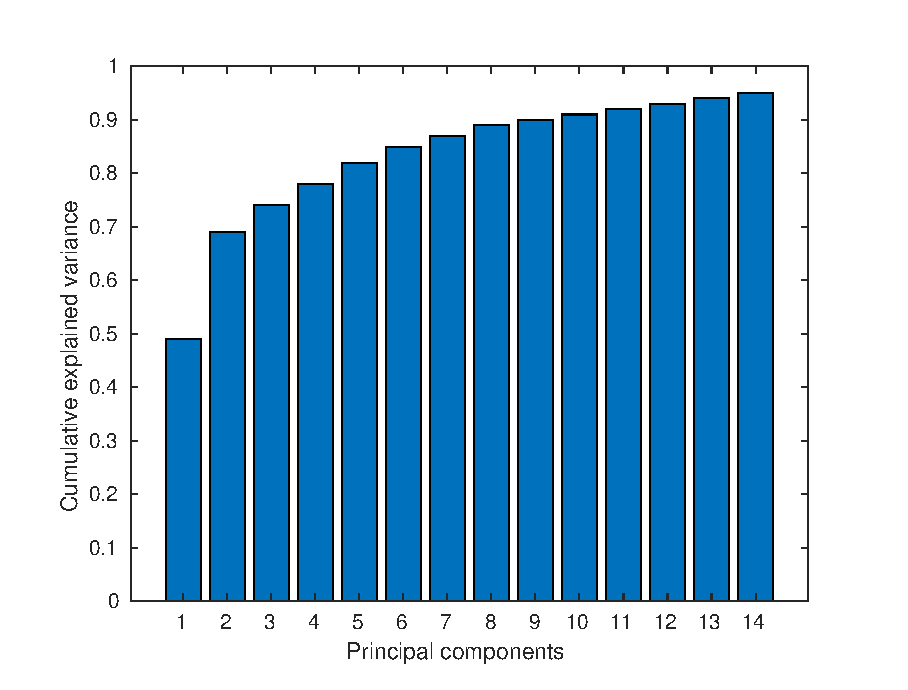
\includegraphics[width=0.6\textwidth]{neural_data_pca1_explained}
		\caption{Cumulative explained variance of the first principal components of the neural data first PCA.}
		\label{fig::neural_data_pca1_explained}
	\end{center}
\end{figure}

The first two principal components explain 69\% of the variance of the neural data.
When plotted in a scatter plot, there are three very obvious clusters (two main at the bottom, one less pronounced on top), as can be seen on Figure~\ref{fig::neural_data_pca1_scatter}.

\begin{figure}[htbp]
	\begin{center}
		\includegraphics[width=0.6\textwidth]{dcsp_2_components_pca}
		\caption{Density-coded scatter plot of the first two components of the neural data first PCA.}
		\label{fig::neural_data_pca1_scatter}
	\end{center}
\end{figure}

That drove us to plot the same data, but this time segregating the samples according to the behavioral categories, as on Figure~\ref{fig::neural_data_pca1_scatter_classes}.

\begin{figure}[htbp]
	\begin{subfigure}{.52\textwidth}
		\begin{center}
			\includesvg[width=\textwidth]{neural_data_pca1_classes}
			\caption{with all the behavioral categories}
		\end{center}
	\end{subfigure}
	\begin{subfigure}{.46\textwidth}
		\begin{center}
			\includesvg[width=\textwidth]{neural_data_pca1_classes_reduced}
			\caption{when regrouping all the grooming categories}
		\end{center}
	\end{subfigure}
	\caption{Behavioral categories segregated scatter plot of the first two components of the neural data first PCA.}
	\label{fig::neural_data_pca1_scatter_classes}
\end{figure}

On Figure~\ref{fig::neural_data_pca1_scatter_classes}, it becomes clear that the two main clusters identified on Figure~\ref{fig::neural_data_pca1_scatter} correspond to actual behavioral categories (respectively resting and walking).
The third cluster however, the one less pronounced on Figure~\ref{fig::neural_data_pca1_scatter}, does not match a specific category.
Rather, it seems that a lot of behaviors can fall in that region of the scatter plot.
When merging all the grooming and pushing behaviors in one unique behavior, it still is not enough to allow for a good bijective mapping:

\begin{itemize}
	\item a point in either bottom clusters allow to identify either walking or resting behaviors,
	\item a point somewhere else on the plot doesn't allow for behavioral discrimination,
	\item and more importantly, choosing a category (any category) does not allow to infer the position of the sample on the scatter plot.
\end{itemize}

However, it still means that some neurons exhibit similar activity when the fly performs either walking or resting.
One benefit of such a redundancy could be a robustness to perturbation when transmitting neural information.

\vspace{\baselineskip}
 
Further manipulation with the application of t-SNE on top of the first PCA lead to the results displayed on Figure~\ref{fig::neural_data_tsne1_scatter}.

\begin{figure}[htbp]
	\begin{center}
		\includegraphics[width=0.6\textwidth]{dcsp_tsne_2_components_pca}
		\caption{Density-coded scatter plot of the t-SNE obtained from the neural data first PCA.}
		\label{fig::neural_data_tsne1_scatter}
	\end{center}
\end{figure}

Unfortunately, it is not a very useful visualization of the data.

\subsubsection{Each neuron as a sample, and each time point as a feature}

Then, we tried to apply the PCA on the neural data again, but the other way round: each neuron as a sample, and each time point as a feature.
Because there are 12 trials, and 4040 time points per trials (so 48480 time points in total), it is necessary for that PCA to reduce the number of time points.
Indeed, viewing the data with this features / samples perspective would not make sense if there were 48480 dimensions and only 123 samples, that would make it a very sparse dataset.
Thus, the data was first averaged over each trial, so that there is only 12 samples left.
The scatter plot of that second PCA is displayed on Figure~\ref{fig::neural_data_pca2_scatter}.

\begin{figure}[htbp]
	\begin{center}
		\includesvg[width=0.6\textwidth]{neural_data_pca2_scatter}
		\caption{Density-coded scatter plot of the neural data second PCA.}
		\label{fig::neural_data_pca2_scatter}
	\end{center}
\end{figure}

Afterwards, another t-SNE was applied to try and see if that leads to interesting results.
They are displayed on Figure~\ref{fig::neural_data_tsne2_scatter}.

\begin{figure}[htbp]
	\begin{subfigure}{.49\textwidth}
		\begin{center}
			\includesvg[width=\textwidth]{neural_data_tsne2_scatter_density}
			\caption{density-coded visualization}
		\end{center}
	\end{subfigure}
	\begin{subfigure}{.49\textwidth}
		\begin{center}
			\includesvg[width=\textwidth]{neural_data_tsne2_scatter_kmeans}
			\caption{k-means clustering}
		\end{center}
	\end{subfigure}
	\caption{Scatter plot of the t-SNE obtained with the neural data second PCA.}
	\label{fig::neural_data_tsne2_scatter}
\end{figure}

We observe three clusters, which means that we have essentially clustered neurons that exhibit correlation in their temporal behavior.

\newpage

	\section{Classification}

\subsection{Behavioral data classification}

The next step in the mini-project was to try and see whether there was a relationship between the three datasets that would allow for behavioral classification.
For this, we used a supervised learning algorithm with the behavioral categories as the discrete target classes.
The algorithm used was a Random Forest Classifier (RFC), as it is not prone to over-fitting, and since decision trees are very simple algorithmically speaking.
An RFC consists of multiple different decision trees merged to get more accurate results.

\vspace{\baselineskip}

The RFC was based on the wavelet angles in order to classify manual behaviors.
We used 25 wavelet features from the joint angles, with frequencies between 1 and \SI{50}{\hertz}.
The resulting classifier displayed an accuracy of around 99.1\% on a test set of the manually predicted data with which it was trained and 77.8\% on the predicted labels column from the initial dataset.
The three most important features in the decision tree were:
\begin{itemize}
	\item the left front leg Coxa roll angle,
	\item followed by the left front leg Coxa pitch angle,
	\item and the left front leg Femur pitch angle.
\end{itemize}

All three features are anatomically located at the base of the fly's leg (see Figure~\ref{fig::drosophila_anatomy}), and probably allow the discrimination between the resting and walking behaviors (the most frequent behaviors). As we are only classyfing behaviors based on joint angles this classifier could be used in other flies.

\begin{figure}[htbp]
	\begin{center}
		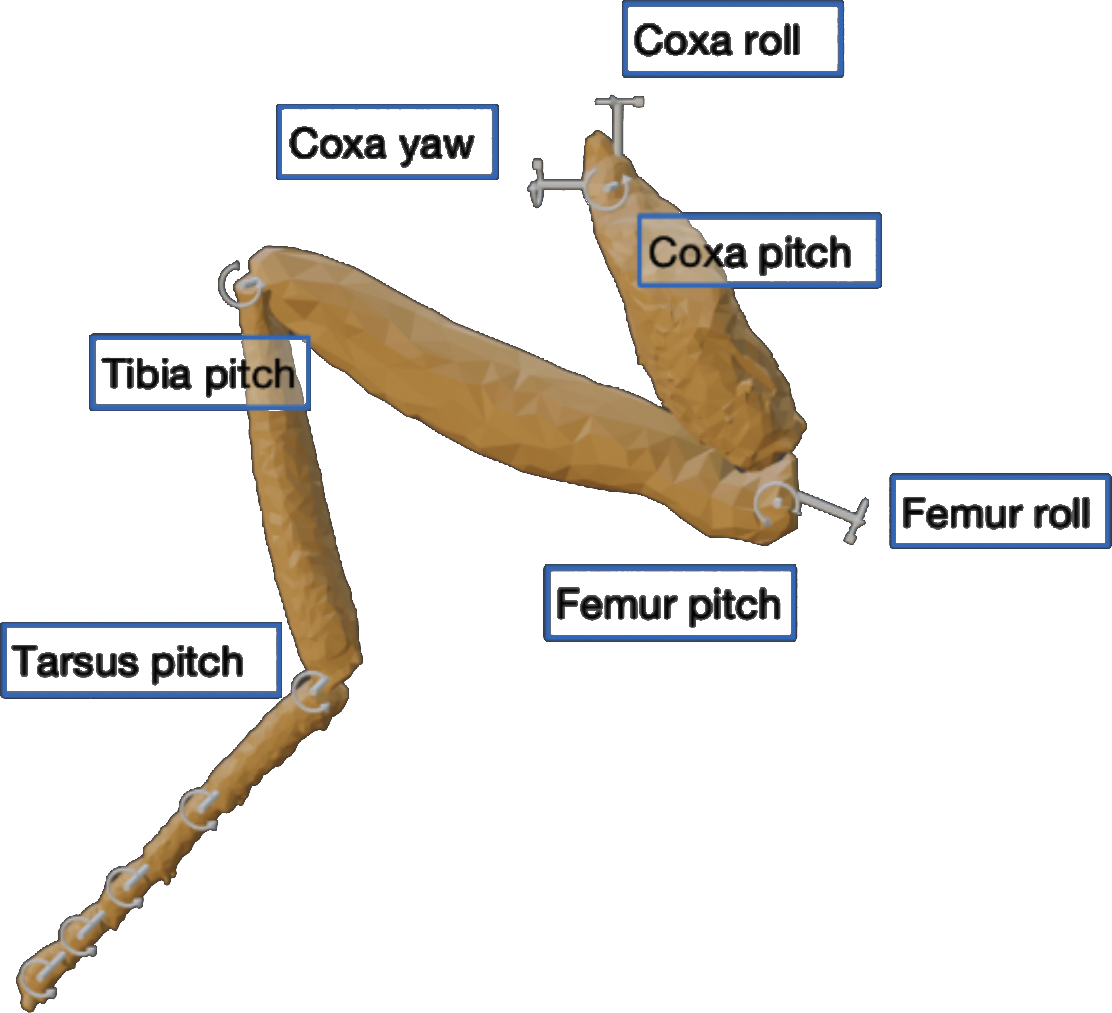
\includegraphics[width=0.4\textwidth]{drosophila_anatomy}
		\caption{The seven joint angles of the \textit{Drosophila} leg segments.}
		\label{fig::drosophila_anatomy}
	\end{center}
\end{figure}

\subsection{Identifying correlations between individual neurons}

In order to try and identify correlation between individual neurons, we normalized the neural dataset to allow comparison between them.
For this we used the z-score.
It corresponds to how many standard deviation from the average a single sample of the signal is.

\vspace{\baselineskip}

After having standardized the neuronal data, we first computed the average activity in all neurons during the different behaviors to see whether some behaviors were triggering higher or lower activity in the neurons. But as can be seen on Figure~\ref{fig::mean_neuron_behav_matrix}, this is not the case. 

\begin{figure}[htbp]
	\begin{center}
		\includesvg[width=0.7\textwidth]{mean_neuron_behav_matrix}
	\end{center}
	\caption{Box plot of average activity for all neurons across the different behaviors.}
	\label{fig::mean_neuron_behav_matrix}
\end{figure}

Then, in order to have a visual representation of specific neural activity, we plotted a matrix of the neurons and their activity levels, which is displayed on Figure~\ref{fig::neuron_behav_matrix}.

\begin{figure}[htbp]
	\begin{center}
		\includesvg[width=0.7\textwidth]{neuron_behav_matrix}
	\end{center}
	\caption{Matrix of the neurons and their relative activity across the different behaviors.}
	\label{fig::neuron_behav_matrix}
\end{figure}

The matrix does not give much insight about a possible higher neural activity given a specific behavior.
Although we can see some higher activity in neurons for certain behaviors, we cannot conclude anything from the matrix.

This prompted us to us to turn towards statistical tools to try and discover correlation between behavior and neural activity.

\vspace{\baselineskip}

For this we used an ANOVA test combined with a Tukey test.
The ANOVA test is a generalization of the t-test, and measures whether two or more distributions have similar means or not.
This is useful for the behavioral data, because there are more than two behavioral categories.

\vspace{\baselineskip}

After the analysis of variance, we tested whether the difference between two behaviors was significant at a 5\% level with a Tukey test.
This test takes the ANOVA significant output and finds out which specific distributions are different by comparing all possible pairs.
The goal was to look for neurons that, for a given behavior, have a significantly different activity than with all other behaviors, at a 5\% level.
The results presented in Table~\ref{tab::statistical_table} are those of such neurons, with the respective associated behavior.

\begin{table}[htbp]
	\sffamily
	\arrayrulecolor{white}
	\arrayrulewidth=1pt
	\renewcommand{\arraystretch}{1.5}
	\rowcolors[\hline]{1}{.!50!White}{}
	\centering
	\begin{tabular}{@{} B|A @{}}
		\cellcolor{ForestGreen}\arraycolor{White}\bfseries Neuron &
		\cellcolor{ForestGreen}\arraycolor{White}\bfseries Behavior \\   
		\arraycolor{Black}
		2 & resting \\
		3 & resting \\
		62 & resting \\
		80 & resting \\
		81 & resting \\
		25 & foreleg grooming \\
		36 & foreleg grooming \\
		42 & abdominal pushing \\
		71 & abdominal pushing \\
		86 & abdominal pushing \\
		109 & abdominal pushing \\
		122 & abdominal pushing \\
		113 & antennal pushing \\
		122 & abdominal grooming \\
	\end{tabular}
	\caption{Neurons exhibiting a significant difference in activity compared with the other neurons when the fly performs the specified associated behavior.}
	\label{tab::statistical_table}
\end{table}

With these results, the next step is to group them by significant behavior, and plot them against time, like on Figures~\ref{fig::trial_7_resting} and~\ref{fig::trial_7_antennal_grooming}.

\begin{figure}[htbp]
	\begin{center}
		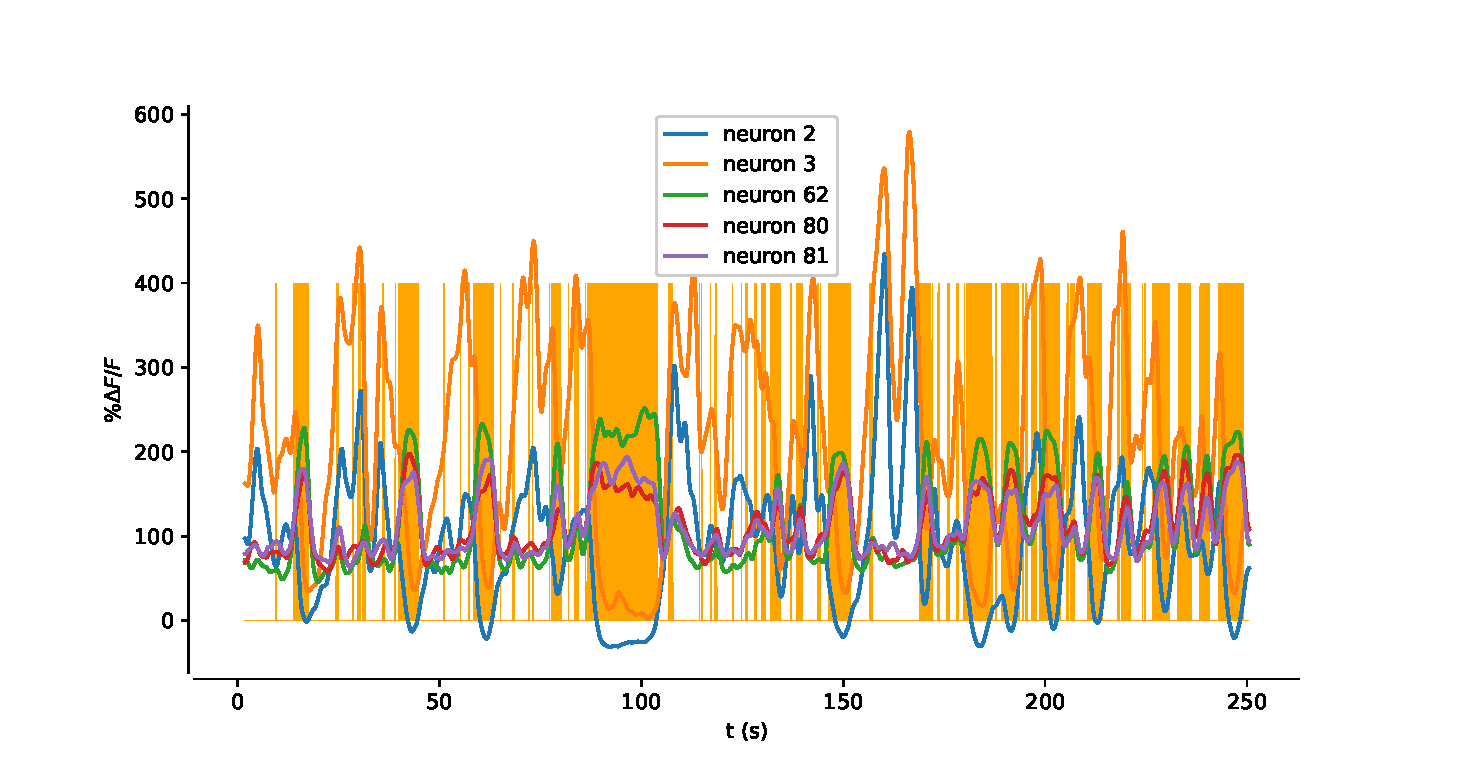
\includegraphics[width=\textwidth]{trial_7_resting}
	\end{center}
	\caption{Neural activity for trial 7, resting state in orange overlay.}
	\label{fig::trial_7_resting}
\end{figure}

\begin{figure}[htbp]
	\begin{center}
		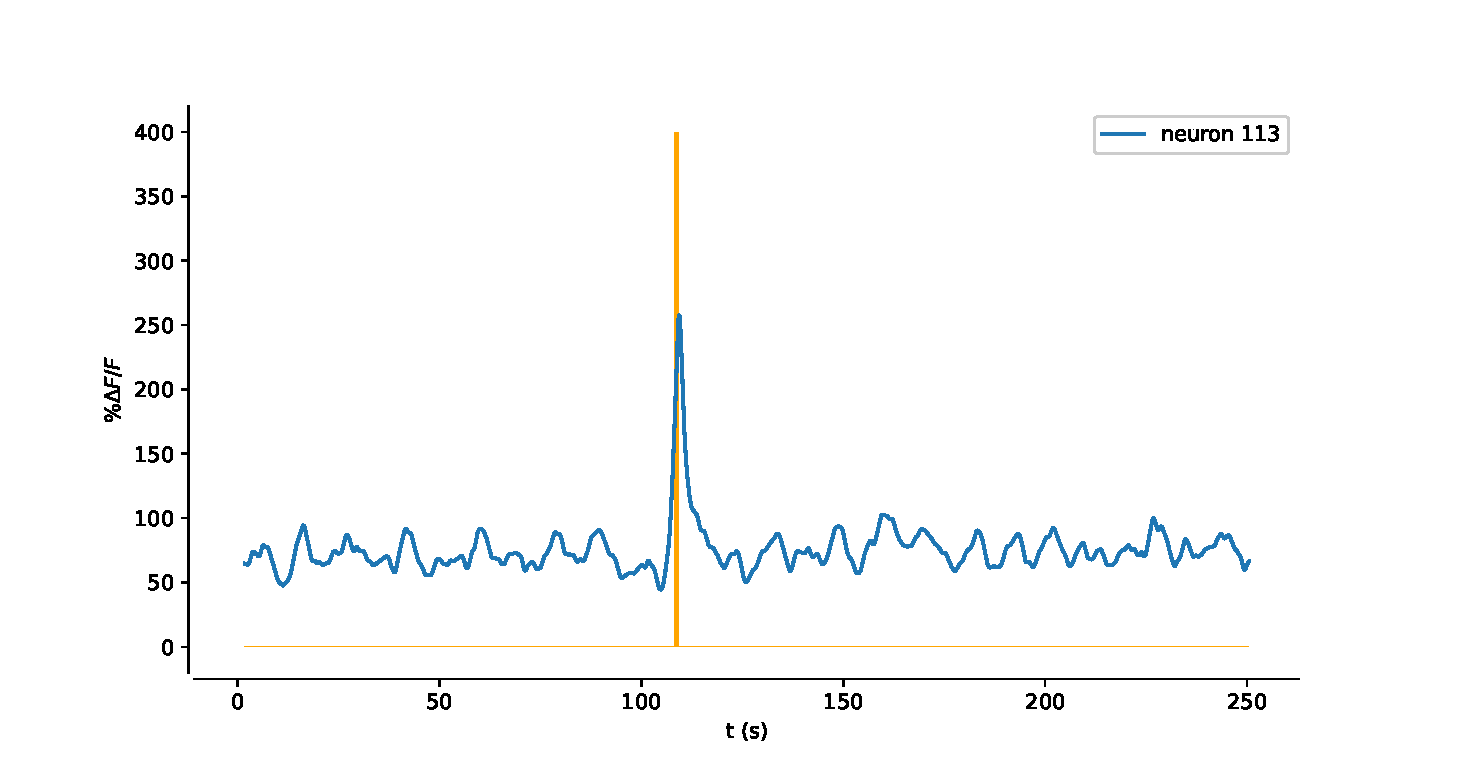
\includegraphics[width=\textwidth]{trial_7_antennal_grooming}
	\end{center}
	\caption{Neuron 113 activity for trial 7, antennal grooming state in orange overlay.}
	\label{fig::trial_7_antennal_grooming}
\end{figure}

We already saw that several behaviors are seldom exhibited by the fly.
This means that the respective data risks being sparse.
For example, for the walking behavior, 58 out of the 123 neurons exhibit a significantly different activity than for the other behaviors, except for hind leg grooming.
However, hind leg grooming is a comparatively rare behavior, that happens only twice in the downsampled behavioral dataset.
Thus, if it were removed from the analysis, the walking behavior could be taken into account.
Here, analyzing 58 additional neurons individually might not be the most effective method, so they were still excluded from Table~\ref{tab::statistical_table}.
The 58 neurons concerned are neurons 2, 5, 7, 9, 10, 11, 12, 20, 21, 23, 25, 26, 29, 30, 31, 32, 34, 36, 38, 39, 41, 48, 49, 51, 55, 58, 59, 61, 62, 63, 65, 68, 69, 70, 71, 73, 76, 78, 79, 82, 85, 86, 89, 91, 92, 94, 95, 97, 99, 101, 102, 105, 106, 114, 116, 117, 121 and 122.

\vspace{\baselineskip}

Then, the Spearman's correlation coefficient between neural data and joint angles was studied.
Joint angles were selected as opposed to joint position, because it was shown earlier that there they are more important for behavioral analysis.
Spearman's correlation coefficient is a method that aims to find a statistical dependence between the ranking of two variables.
In Table~\ref{tab::spearman_table}, the Spearman's correlation coefficients greater than 0.5 or lesser than -0.5 are retained, to observe moderately to highly correlated joint angles to neural data, keeping only the ones where the p-value of that correlation was lower than 5\%.

\begin{table}[htbp]
	\sffamily
	\arrayrulecolor{white}
	\arrayrulewidth=1pt
	\renewcommand{\arraystretch}{1.5}
	\rowcolors[\hline]{1}{.!50!White}{}
	\centering
	\begin{tabular}{@{} B|A|A @{}}
		\cellcolor{ForestGreen}\arraycolor{White}\bfseries Neuron &
		\cellcolor{ForestGreen}\arraycolor{White}\bfseries Angle &
		\cellcolor{ForestGreen}\arraycolor{White}\bfseries Correlation \\   
		\arraycolor{Black}
		36 & LM leg Femur & 0.63 \\
		25 & LM leg Femur & 0.61 \\
		101 & RH leg Coxa roll & 0.58 \\
		117 & LM leg Femur & 0.57 \\
		65 & LM leg Femur & 0.55 \\
		102 & LM leg Femur & 0.55 \\
		63 & LM leg Femur & 0.55 \\
		25 & LF leg Femur & 0.50 \\
		36 & RM leg Femur & 0.50 \\
		36 & LF leg Femur & 0.50 \\
		36 & LM leg Tarsus & -0.57 \\
		25 & LM leg Tarsus & -0.57 \\
		25 & RH leg Coxa roll & -0.55 \\
		102 & RH leg Coxa roll & -0.52 \\
		20 & RH leg Coxa roll & -0.52 \\
		117 & LM leg Tarsus & -0.51 \\
		36 & RM leg Tarsus & -0.50 \\
	\end{tabular}
	\caption{Spearman's correlation coefficients for correlated joint angles with the neural data.}
	\label{tab::spearman_table}
\end{table}

On Figure~\ref{fig::spearman_neuron_36} is plotted the biggest Spearman's correlation coefficient, which is for neuron 36 and the left medial Femur angle, with a coefficient of 0.63, $p<0.05$.

\begin{figure}[htbp]
	\begin{center}
		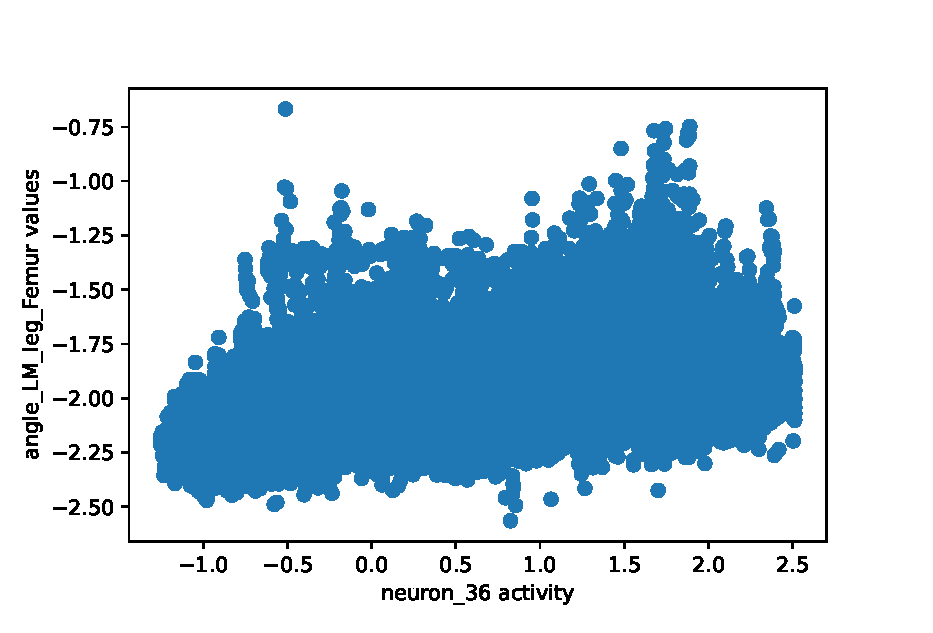
\includegraphics[width=0.6\textwidth]{spearman_neuron_36}
	\end{center}
	\caption{Spearman's positive correlation coefficient of 0.63, $p<0.05$ for neuron 36 for the left medial Femur.}
	\label{fig::spearman_neuron_36}
\end{figure}

The highest correlation is not very high.
A possible explanation is that DNs are more correlated to behavioral categories than to joint angles.
From a neural and anatomical perspective, it could be explained if those neurons encode entire behaviors rather than joint angles, the latter being a result in a process involving many different neuron contributions. 

\subsection{Predicting behavior from neural activity}

\subsubsection{Logistic regression with one behavior: walking}

Then, a logistic regression was performed on the neural data points in order to classify behaviors.
Logistic regression is a method that classify binary categorical outputs, e.g. walking or not walking.
It is based on a logistic function that smoothly varies from 0 to 1 depending on the input. 
The first logistic regression done was performed on each neural activity separately as input, with the output being whether or not the fly exhibit the walking behavior. Table~\ref{tab::lr_single_neuron} summarizes the results of the regression with the 10 most predictive neurons with their maximum accuracy.

\begin{table}[htbp]
	\sffamily
	\arrayrulecolor{white}
	\arrayrulewidth=1pt
	\renewcommand{\arraystretch}{1.5}
	\rowcolors[\hline]{1}{.!50!White}{}
	\centering
	\begin{tabular}{@{} B|B @{}}
		\cellcolor{ForestGreen}\arraycolor{White}\bfseries Neuron &
		\cellcolor{ForestGreen}\arraycolor{White}\bfseries Accuracy \\   
		\arraycolor{Black}
		32 		& 0.788		\\
		38		& 0.787		\\
		99		& 0.785		\\
		28 		& 0.784 	\\
		12 		& 0.779 	\\
		51		& 0.774		\\
		93		& 0.773		\\
		62		& 0.772		\\
		48		& 0.771 	\\
		5		& 0.768		\\
		All 	& 0.853
	\end{tabular}
	\caption{Logistic regression accuracy for the 10 most accurate neurons for the walking behavior.}
	\label{tab::lr_single_neuron}
\end{table}

Table~\ref{tab::lr_single_neuron} shows that looking for the specific neurons that best classify for the walking behavior provides us with approximately 40 with an accuracy greater than 70\%.
If instead of looking for a specific neuron, we look at all the neurons together, we can classify for the walking behavior with an accuracy of 85\%.
This let's us think that the walking behavior is not controlled by only one neuron, but several, which is consistent with the results of the ANOVA.

\vspace{\baselineskip}

On Figures~\ref{fig::ow_neuron_32} and~\ref{fig::ow_neuron_38} are displayed the two most relevant neurons found in Table~\ref{tab::lr_single_neuron}.
For both, there is a definite increase in neural activity during the walking motion, and a definite decrease in activity during resting.

\subsubsection{Logistic regression with multiple behaviors}

The logistic regression was then applied to all neural activity in order to classify all the neurons.
The accuracy found for this regression is 0.806.
Table~\ref{tab::lr_multiple_neuron} summarizes the 10 most important neurons for each behavior.

\begin{table}[htbp]
	\sffamily
	\arrayrulecolor{white}
	\arrayrulewidth=1pt
	\renewcommand{\arraystretch}{1.5}
	\rowcolors[\hline]{1}{.!50!White}{}
	\centering
	\begin{tabular}{@{} A|C|C|C|C|C|C|C|C|C|C @{}}
		\cellcolor{ForestGreen}\arraycolor{White}\bfseries Neuron &
		\cellcolor{ForestGreen}\arraycolor{White}\bfseries 1 &
		\cellcolor{ForestGreen}\arraycolor{White}\bfseries 2 &
		\cellcolor{ForestGreen}\arraycolor{White}\bfseries 3 &
		\cellcolor{ForestGreen}\arraycolor{White}\bfseries 4 &
		\cellcolor{ForestGreen}\arraycolor{White}\bfseries 5 &
		\cellcolor{ForestGreen}\arraycolor{White}\bfseries 6 &
		\cellcolor{ForestGreen}\arraycolor{White}\bfseries 7 &
		\cellcolor{ForestGreen}\arraycolor{White}\bfseries 8 &
		\cellcolor{ForestGreen}\arraycolor{White}\bfseries 9 &
		\cellcolor{ForestGreen}\arraycolor{White}\bfseries 10 \\   
		\arraycolor{Black}
		Resting 				& 0 & 62 & 109 & 48 & 100 & 101	& 73 & 30 & 41 & 36 \\
		Walking					& 28 & 109 & 100 & 103 & 117 & 48 & 101 & 23 & 39 & 38 \\
		Abdominal pushing		& 22 & 7 & 8 & 20 & 40 & 116 & 105 & 30 & 23 & 42 \\
		Anterior grooming 		& 34 & 89 & 99 & 84 & 44 & 38 & 100 & 51 & 65 & 119 \\
		Posterior grooming 		& 118 & 120 & 47 & 33 & 43 & 112 & 108 & 39 & 93 & 89 \\
		Foreleg grooming		& 85 & 89 & 51 & 61 & 44 & 102 & 2 & 99 & 0 & 81 \\
		Abdominal grooming		& 50 & 87 & 43 & 83 & 7 & 107 & 60 & 52 & 90 & 95 \\
		Hind leg grooming		& 27 & 74 & 9 & 122 & 76 & 107 & 22 & 98 & 58 & 93 \\
		Antennal grooming		& 99 & 21 & 34 & 89 & 41 & 34 & 91 & 103 & 65 & 32 \\
	\end{tabular}
	\caption{The ten most accurate neurons for each behavior from logistic regression accuracy.}
	\label{tab::lr_multiple_neuron}
\end{table}

It can be seen on Table~\ref{tab::lr_multiple_neuron} that a lot of neurons found in the walking behavior classification are also overall important for the classification when taking into account all behaviors, like for example neurons 38 and 28.

\vspace{\baselineskip}

On Figures~\ref{fig::ow_neuron_32},~\ref{fig::ow_neuron_38},~\ref{fig::fr_neuron_93} and~\ref{fig::rf_neuron_62}, the neural activity was plotted with the resting and walking states in overlay. As already stated, for each there is a definite increase in neural activity during the walking motion, and a definite decrease in activity during resting.

\begin{figure}[hbtp]
	\begin{center}
		\includesvg[width =\textwidth]{neuron_32}
	\end{center}
	\caption{Neuron 32 activity, resting state in orange overlay, walking state in blue overlay.}
	\label{fig::ow_neuron_32}
\end{figure}

\begin{figure}[hbtp]
	\begin{center}
		\includesvg[width =\textwidth]{neuron_38}
	\end{center}
	\caption{Neuron 38 activity, resting state in orange overlay, walking state in blue overlay.}
	\label{fig::ow_neuron_38}
\end{figure}

\begin{figure}[hbtp]
	\begin{center}
		\includesvg[width =\textwidth]{neuron_93}
	\end{center}
	\caption{Neuron 93 activity, resting state in orange overlay, walking state in blue overlay.}
	\label{fig::fr_neuron_93}
\end{figure}

\begin{figure}[hbtp]
	\begin{center}
		\includesvg[width =\textwidth]{neuron_62}
	\end{center}
	\caption{Neuron 62 activity, resting state in orange overlay, walking state in blue overlay.}
	\label{fig::rf_neuron_62}
\end{figure}

It can be observed on these Figures that neural activity is a very good predictor for the walking and resting behaviors.

\subsubsection{Random forest classifier}

To compare the results found with the logistic regression, a random forest classifier was trained.
It was found to have an accuracy of 87.5\%.
The ten most important neurons for the classifier are neurons 93, 62, 60, 103, 28, 81, 29, 23, 51 and 32.

\newpage


	\section{Discussions}

Several results of this mini-project were particularly interesting.

\vspace{\baselineskip}

The first one is on Figure~\ref{fig::neural_data_pca1_scatter_classes}, where it can be seen that the walking and resting behavioral categories of \textit{Drosophila} cluster quite nicely when a PCA is performed on the neural activity of the DNs, which means that DNs neural activity can at least partially predict for these behaviors.

\vspace{\baselineskip}

Another interesting result is the fact that the logistic regression leads to a better accuracy when classifying for one categorical behavior than for all behaviors simultaneously.
Also worthy of note is that on Figures~\ref{fig::ow_neuron_32},~\ref{fig::ow_neuron_38},~\ref{fig::fr_neuron_93} and~\ref{fig::rf_neuron_62}, we only tried to classify for the walking and resting behaviors.
This is in part motivated by the fact that walking and resting behaviors account for approximately 80 to 90\% of the fly's behavior; and in part because since the beginning of the project, walking and resting behaviors stand out better and are better clustered for, classified or otherwise predicted.

\newpage

	\section{Conclusion}

This project was very interesting.
The nature of the data and of the assignment itself -- the fact that we were asked to be exploratory in our analysis of the data made it unique in that we had to try and fail at discovering relationships and meanings before we could obtain something from the data.

\vspace{\baselineskip}

Another interesting thing to note was that the predicted behavioral labels provided in the initial dataset were unreliable.
The main problem was that among the predicted behaviors, there were some that weren't exhibited by the fly, and thus were not appearing on the manually labeled behaviors, because when downsampling, both the predicted and manual labels were taken into account.
A better labeling of the categorical behavior would not categorize behaviors that the subject does not exhibit (which was the issue with the predicted labeling).

\vspace{\baselineskip}

This leads to other considerations, like how precisely within the experiment are the behaviors categorized.
Indeed, on Figure~\ref{fig::neural_data_pca1_scatter_classes}, we plot with and without merging the grooming and pushing categories.
In the experiment design, how is it decided how many categories to choose, and which ones?
Does the walking get to be further broken down between turning left, turning right and walking straight?
Should all the groomings be merged?
Those are valid design choices to wonder about, and the answer is not straightforward, because the best categorization can only be known after the results are understood (which is not a very causal experiment design).

\vspace{\baselineskip}

Thus, a first major improvement of the data labeling process would be to not predict the labels, and to make a unique person label all the dataset, to reduce variation in how the edge behaviors are labeled.
Further improvement would be to have a second person verifying the labeling.

\vspace{\baselineskip}

On the bright side, the analysis of the neural data, and in particular the logistic regressions brought forward so strong insights on the data that it was sufficient to notice that trial 4 had been (manually) mislabeled.
This is strong evidence that the results brought by that particular piece of analysis are actually very robust and significant.

\vspace{\baselineskip}

One tool that we did not have to use but was very beneficial for our work was the pose-estimation algorithm \textit{DeepFly3D} with which all joint angles and positions were estimated.
This algorithm is really speeding up the analysis as no manual labeling of positions and angles needs to be done.  

\vspace{\baselineskip}

With this analysis, even though we found very interesting correlation between neural and behavioral data, we cannot infer causation.
Indeed, this is an observational study.
It allows to posit hypotheses on hypothetical links between DNs and high-level fly behavior, but to confirm those hypotheses, experimental studies need to be done, for example with genetic manipulations.


	%%%%%%%%%%%%%%%
	%% BIBLIOGRAPHY
	%%%%%%%%%%%%%%%
	\newpage
	\section*{Bibliography} % to add a section-like unnumbered title
	\addcontentsline{toc}{section}{Bibliography} % to add said title to the toc
	\markboth{Bibliography}{Bibliography} % to modify the header
	\printbibliography[
	heading=subbibintoc,
	type=article,
	title={Articles}
	]

\end{document}